%%%%%%%%%%%%%%%%%%%%%%%%%%%%%%%%%%%%%%%%%%%%%%%%%%%%%%%%%%%%%%%%%%%%%%%%%%%
%                                                                         %
%			TEMPLATE LATEX PER TESI                                       %
%			______________                                                %
%                                                                         %
%           Ultima revisione: 24 giugno 2019                              %
%           Revisori: G.Presti; L.A.Ludovico; F. Avanzini                 %
%                                                                         %
%%%%%%%%%%%%%%%%%%%%%%%%%%%%%%%%%%%%%%%%%%%%%%%%%%%%%%%%%%%%%%%%%%%%%%%%%%%

\documentclass[12pt,italian, twoside]{report}
\usepackage{tesi}
%
%			INFORMAZIONI SULLA TESI
%			DA COMPILARE!
%

% CORSO DI LAUREA:
\def\myCDL{Master's in\\Data Science and Economics}

% TITOLO TESI:
\def\myTitle{TRADITIONAL VS MACHINCE LEARNING MODELS{:}\\
	\small{The Problem of Macroeconomic Forecasting}}
% AUTORE:
\def\myName{Sainey Manga}
\def\myMat{Matr. Nr. 943874}

% RELATORE E CORRELATORE:
\def\myRefereeA{Prof. Silvia Salini}
\def\myRefereeB{Prof. Giancarlo Manzi}

% ANNO ACCADEMICO
\def\myYY{2021-2022}

% Il seguente comando introduce un elenco delle figure dopo l'indice (facoltativo)
%\figurespagetrue

% Il seguente comando introduce un elenco delle tabelle dopo l'indice (facoltativo)
%\tablespagetrue

%
%			PREAMBOLO
%			Inserire qui eventuali package da includere o definizioni di comandi personalizzati
%

% Package di formato
\usepackage[a4paper]{geometry}		% Formato del foglio
\usepackage[english]{babel}			% Supporto per l'italiano
\usepackage[utf8]{inputenc}			% Supporto per UTF-8
\usepackage[a-1b]{pdfx}			% File conforme allo standard PDF-A (obbligatorio per la consegna)

% Package per la grafica
\usepackage{graphicx}				% Funzioni avanzate per le immagini
\usepackage{hologo}					% Bibtex logo with \hologo{BibTeX}
%\usepackage{epsfig}				% Permette immagini in EPS
%\usepackage{xcolor}				% Gestione avanzata dei colori

% Package tipografici
\usepackage{amssymb,amsmath,amsthm} % Simboli matematici
\usepackage{listings}				% Scrittura di codice

% Package ipertesto
\usepackage{url}					% Visualizza e rendere interattii gli URL
\usepackage{hyperref}				% Rende interattivi i collegamenti interni
%\linespread{1.5}

\begin{document}
% Creazione automatica del frontespizio
\frontespizio
\beforepreface

% 
%			PAGINA DI DEDICA E/O CITAZIONE
%			facoltativa, questa è l'unica cosa che dovete formattare a mano, un po' come vi pare
%
\iffalse
{\raggedright \large \sl Questo lavoro \`{e} dedicato a tutti gli studenti\\
	
	\vspace{2cm}
	
	``Io studio,\\ma studiate pure voi,\\che se studio solo io non serve a un c\dots o''
	
	\bigskip
	
	\--- Gli scarabocchi di Maicol \& Mirco\\
  
	\vspace{2cm}
	
	``No tale is so good \\ that it can't be spoiled \\ in the telling''
	
	\bigskip
	
	\--- Proverbio\\}
  \fi
% 
%			PREFAZIONE (facoltativa)
%

%\prefacesection{Prefazione}
%Le prefazioni non sono molto comuni, tuttavia a volte capita che qualcuno voglia dire qualcosa che esuli dal lavoro in s\'e (come un meta-commento sull'elaborato), o voglia fornire informazioni riguardanti l'eventuale progetto entro cui la tesi si colloca (in questo caso \`e probabile che sia il relatore a scrivere questa parte).

%
%			RINGRAZIAMENTI (facoltativi)
%

\prefacesection{Acknowledgement}
Praises and salutations are due to God, without whom nothing would have been possible. I would like to thank my supervisor, Prof. Silvia Salini for her input throughout, and accepting to supervise me in spite having a plethora of students to supervise. I extent my appreciation to Prof. Giancarlo Manzi for being my co-supervisor.
To my parents and siblings whose unreserved love and support pushed me thus far, I say thank you. I thank my Professors and course mates from the DSE program, especially Hoai Nam Nguyen whom I had worked with in so many projects. Special thanks to Mr. Mamut Jagne for being available to review my work at any point before sending it to my supervisor. To all that contributed in a way or another in making this work a complete project, I say “Grazie”.

\prefacesection{Abbreviation}
\textbf{ML} Machine Learning
\\
\textbf{VAR} Vector Autoregressive Model\\
\textbf{ARIMA}  Autoregressive Integrated moving average\\
\textbf{RF} Random Forest Model
\\
\textbf{EN} Elastic Net Model
\\
\textbf{GDP} Gross Domestic Product\\
\textbf{SVM} Support vector Machine Model\\
\textbf{LSTM} Long-Short Term Memory Model\\
\textbf{MICE} Multiple Imputation by Chained Equation\\
\textbf{GDP} Gross Domestic Product
\\


\prefacesection{Abstract}
This research makes a comparison between traditional and machine learning models in terms of macroeconomic forecasting in low-income economies, using Real GDP growth of The Gambia as a case study. We implemented the Vector Autoregressive model as our benchmark representing the traditional models, and Random Forest, Elastic Net, Support Vector Machine and Long-Short Term Memory models representing the machine learning models. These models were fitted on two different datasets generated from the imputation of missing values. The study further implemented the Shapley values framework to perform inferential analysis for the machine learning models, choosing the Random Forest model. The study finds that machine learning models can outperform traditional models and that methods used in imputing the missing values of a dataset can influence the performance of a model. Models like Long-Short Term Memory do not perform well on a small sample size and was outperformed by Vector Autoregressive model. Machine learning models can be used for causal inference through the use of Shapley values, but with limitations. 



%
%			Creazione automatica dell'indice
%

\afterpreface
% 
%			CAPITOLO 1: Introduzione o Abstract
% 

\chapter{INTRODUCTION}
\label{cap:introduction}

Forecasting is one of the most challenging tasks in the field of economics. Policy makers rely so much on economic forecasts to guide their policy frameworks. These policies shape the economy in the short and long run thereby demanding accurate and precise forecasting. Macroeconomics is one area of economics that relies heavily on forecasting, where the forecasted figures signal the direction of the economy in that period. Policy makers would react to these signals as research would also reveal what might be possibly responsible for the said signals. If the fall in output can be discovered in time by the decision-makers, adjustments on monetary policies could be taken with the fiscal policies to avert the recession or better still reduce the impacts on the real economy.
\\
The International Monetary Fund (IMF), World Bank (WB) and various national statistics institutions are known for making quarterly and yearly forecasting of economic indicators. These forecast values often variate with actual release values, sometimes with better accuracy. A typical example of the failure of the forecasting community is that the economic recession of 2008/2009 was not predicted earlier. After the recent crises in the economy worldwide, the issue of forecasting output gaps is very topical and has significant implications in terms of economic policy. Timely warning of an upcoming output downturn (recession) is of course extremely important to policymakers as they can swiftly adjust fiscal and monetary policy to either steer the economy away from a recession or dampen its impact to the real economy. \\ 
There are some general concerns which emerge from the literature on forecasting accuracy, especially with respect to the long-term predictions for macroeconomic variables. Macroeconomic forecasters have traditionally relied upon two different approaches – structural and non-structural (Diebold, 1998). The structural approach is guided by economic theory for model specification while the non-structural approach focuses on exploiting the specific properties of the underlying data without explicitly relying on any economic theory. Non-structural models weigh more importance to predictive accuracy over causal inference and are useful for short-term unconditional forecasting. Time-series models, like the univariate autoregressive integrated moving average (ARIMA) or the multivariate vector autoregression (VAR) models, are usually the preferred non-structural models (Pescatori etal, 2011). Linearity in parameters is a key assumption of such time-series models. However, as it was observed during the 1980s and 1990s, linear models failed to identify macroeconomic business cycles, periods of extreme volatility and regime changes which led non-linear models to gain more attention (Sanyal and Roy, 2014). In general, macroeconomic variables do not always display a linear correlation and as such would affect the precision of the forecast values when some predictors have a non-linear correlation with the target variable. Predicting macroeconomic dynamics is challenging. Relationships between variables may not hold over time, and shocks such as recessions or financial crises might lead to a breakdown of previously observed relationships.
\\
Of recent, the field of macroeconomic forecasting has seen a rising wave in the application of ML models due to their predictive power. The goal of this research is to compare between these ML models and traditional models of forecasting. What we refer to as traditional models in this research are the common econometric models used for time series forecasting. ML on the other hand is the study of computer algorithms that can improve automatically through experience and by the use of data. It is seen as a part of artificial intelligence. ML algorithms build a model based on sample data, known as training data, in order to make predictions or decisions without being explicitly programmed to do so. ML approaches are traditionally divided in to supervised, unsupervised and reinforcement learning. We focus on the supervised learning approach, where a model is built upon a set of data that contains both the inputs and the desired outputs. The data is known as training data and consists of a set of training examples. Each training example has one or more inputs and the desired output, also known as a supervisory signal.
\\
Real GDP is a key macroeconomic indicator used for measuring the state of an economy. It enables policymakers to judge whether the economy is expanding or contracting and permits them to make appropriate monetary or fiscal policy decisions accordingly. In that regard, the accurate and timely forecast of GDP growth ahead of the release of official GDP figures is important.\\ 
This paper aims at comparing between the performances of ML models and traditional models in macroeconomic forecasting, using the case study of real GDP growth. We investigated this comparison by forecasting Real GDP growth of the Gambia using twelve predictors. The Gambia is one of the low-income countries where data availability is a big issue, making data driven research more difficult. We have a data set with a small sample size with massive missingness, only two variables are without missing values. As a result, the main idea is to implement two different methods of imputing missing values. We would then keep each result generated through the implementation of each method as a separate data. Each of these two different data sets would be fed to a model each at a time. The two methods used for imputing the missing values of our data are the Multiple Imputation by Chained Equation and the Softimpute methods. We implemented the VAR model which is the benchmark model representing the traditional models class, and RF, EN, SVM and LSTM representing the ML models class. These models are evaluated using RMSE and MAE as the evaluation matrices. To perform causal inference using ML models, the research utilizes the Shapley values framework which has recently been explored as a way of interpreting and extracting individual attribute contribution to the prediction of an ML model.
\\
The paper is organized in the following way: in chapter 2, we have the research question where we discuss the research gap as well as the research questions and how this research contributes to the literature. Chapter 3 discusses the methods applied in this research. It entails an explanation of the data used and the models applied. Chapter 5 discuses and deeply analyzed the results generated by the different models used. Finally, chapter 6 concludes the findings made in this research. We also prepared an Appendix to show all the figures generated from the implementation of our models.




% 
%			CAPITOLO 2: Stato dell'arte
% 

\chapter{RESEARCH QUESTION}
\label{chap:stato_arte}


Recently, the forecasting community explored as an alternative, the use of Machine Learning (ML) and Artificial Intelligence (AI) models to improve the forecast accuracy and narrow down the gap in deviations. This is a growing approach in the macroeconomic forecasting literature. In fact, in conjunction with technological development and the increase in predictive power, ML models have been actively applied in various fields.
\\
There is a good number of research that investigated and compared the performance between the conventional time series models and the ML models. So far, a huge chunk of those body of literature have focused on data-rich economies. ML models are widely believed to be data driven models. There is little research in the literature that tried to apply such investigation in data-poor countries, low-income countries in particular. We have seen papers that investigated these models using South Africa (Martin, 2019, Mulaudzi and Ajoodha, 2020) as a case study and Nigeria as well (Chuku et al. 2017, Oyewale et al. 2019). However, despite these countries being under the category of low-income countries, the data used for their respective papers were relatively sufficient as they have sample size more than a hundred with no reported missing values. According to Jung et al. (2018), their research did not cover low-income economies as data for these economies are only available for shorter time periods and often suffer from missing data, resulting in a prohibitively low number of observations. For them, this was something they looked forward to working in the future. This has been the corner stone of this research the moment we decided to investigate the application of the ML models in forecasting Real GDP growth of The Gambia. For the four months spent on this work, the author did not come across any similar research done using ML models to forecast macroeconomic variables in the Gambia, more so to compare their performances with those of the Traditional models.
\\
This paper aims at comparing the performances of ML models with traditional models in macroeconomic forecasting, using the case study of real GDP growth. We investigated this comparison by forecasting Real GDP growth of the Gambia using twelve predictors. By virtue of our choice, we hope to add to the literature by providing the case study of a data-poor country with missing values. The Gambia is one of the low-income countries where data availability is a big issue, making data driven research more difficult. We would use this constraint to our advantage by exploring techniques of handling missing values in a data set. Basuchoudhary et al (2017) were faced with missingness even though their case study was not a low-income country. We have a data set with a small sample size with massive missingness, only two variables are without missing values. As a result, the main idea is to implement two different methods of imputing missing values. We would then keep each result generated through the implementation of each method as a separate data. Each of these two different data sets would be fed to a model each at a time. Since we have huge missingness, this approach would help us know if the method used to impute the missing values would have an impact on the performance of a model. Based on the main task at hand, the choice of our methods for imputing the missing values was guided by the types of models used for forecasting. i.e a linear and a nonlinear method were used to impute the missing values. The purpose is to know which method is suitable for which class of forecasting models and which method is not suitable.
\\
The research questions investigated in this paper are divided into three folds: The first part would add to the literature by investigating if methods used in imputing missing values could affect the performance of a model, especially when the data suffers massive missingness. Should linear methods be used to impute missing values when forecasting with linear models, and non-linear methods be applied when forecasting with non-linear models? The second part would contribute to the existing literature by investigating and comparing various ML models with conventional time series models in terms of forecasting accuracy.
\\
Despite providing an alternative to the forecasting community, ML Models have been earlier criticized as black boxes. The models would produce high predictive accuracy, but explanation of results was not popular, which makes casual inference difficult. This led to the use of Shapley values to explain the prediction made by ML models. Strumbelj and Kononenko (2010) are some of the notable researchers to adopt this method in trying to explain the prediction of ML models. In order to contribute to the literature, the third research question investigated in this paper attempts to find out if ML models can be used for casual inference through the use of Shapley values, testing for the statistical significance of each feature estimate. We would further study to know if the findings from the Shapley values conform with the intuitions of economic theory. This is due to the criticism that the Shapley values method provides non-intuitive results.  This would provide a conclusion as to whether ML models can completely replace traditional time series models in macroeconomic forecasting.\\
In all, this research would add to the literature by providing a comparison between traditional models and ML models on low-income economies with a small data observation and massive missingness. The research also adds to the small body of literature, the application of such studies in sub-Saharan economies. Another phase of contribution made in this research is the study conducted to know which class of missing values imputation method is suitable for which class of forecasting models and how much influence does the imputation method has on the performance of a model.
The summary of our three research questions are as follows:
\begin{itemize}
\item Can Machine Learning Models outperform conventional models in forecasting Real GDP growth?
\item Does the missing values imputation method affect a model performance?
\item Can Machine Learning Models be useful in causal inference as compared to their counterparts?
\end{itemize}




% 
%			CAPITOLO 3: Tecnologie utilizzate
% 

\chapter{LITERATURE REVIEW}
\label{cap3}

The application of ML models in macroeconomic forecasting is recently and rapidly growing in the literature. An increase in the volume of data available, in addition to improvements in data processing and storage, has created the need to make use of more data-driven modelling techniques as an alternative to conventional forecasting models. This also brought about a comparison between the two classes of models in terms of forecasting accuracy in the literature. Some part of the literature only focused on the accuracy in absolute terms whilst others compared accuracy case-on-case basis.\\
Jaehyun Yoon (2020) presented a method for creating machine learning models, specifically a gradient boosting model and a random forest model, to forecast real GDP growth. The study focused on the real GDP growth of Japan and produced forecasts for the years from 2001 to 2018 using data from the fourth quarter of 1981 up to the second quarter of the year of prediction. In order to compare these models with conventional models, the paper used forecasts by the IMF and Bank of Japan (BOJ) as benchmarks.The machine learning models produced forecasts that are overall more accurate than those produced by the IMF and the BOJ. However, for 2009, a year during which the global economic crisis was on- going, the ML models did not predict the extreme drop in real GDP growth, which was forecasted by the IMF.\\
Forecast performances are sensitive to training and test split specifications and generally ML algorithms are strongly driven by the underlying data. Jin-Kyu Jung et al (2018) suggested that forecasts produced by ML algorithms cannot entirely replace expert forecasting altogether, however, might serve as a valuable additional benchmark when making discretionary decisions about a final economic forecast. To test the strength of the ML approach on crisis induced volatility episodes as well as on advanced economies, they covered as case studies three advanced/G-7 economies (United States, United Kingdom and Germany), together with a diverse set of emerging and developing economies (Mexico, Philippines and Vietnam). They applied the Elastic Net, Super Learner, and RNN algorithms to determine one-step ahead GDP growth forecasts using both set of quarterly and yearly datasets of these various countries. The performances of the ML algorithms were compared to the IMF world economic outlook (WEO) forecasts as benchmark. The study found that in all cases of quarterly data, ML algorithms outperform the WEO forecasts in the test period between 2010 and 2016. The Elastic Net and Super Learner models consistently outperform the benchmark whereas the RNN outperforms WEO forecasts only once in the case of the Philippines. For the case of the annual horizon, forecast performance declined in absolute as well as relative terms when measured against the WEO benchmark. For Spain and Mexico for instance, none of the ML models were able to outperform the WEO forecasts. While their study showed that the three ML algorithms were able to consistently outperform a benchmark forecast performance by the IMF’s WEO forecasts, it suggested that the low number of observations is a challenge that presents itself to most traditional macroeconomic variables in a ML context.
\\
Some studies also suggest that the performance of a model may depend on the nature of the variable of interest, though most macroeconomic variables of an economy entail similar nature. Syed and Lee (2020) focused on forecasting the inflation, GDP growth and the weighted average overnight repurchase rate in Pakistan using 161 predictors over 12 month forecast horizon. They used the naïve mean model and the AR model as benchmarks and compared their forecasting performance against the dynamic factor model (DFM) and sophisticated ML methods such as the Ridge regression, the LASSO and the Elastic net. Their results showed that inflation is best forecasted by the AR model, but the DFM and LASSO models best forecast the GDP growth. Overall, their study concluded that the ML approaches perform better than the DFM in presence of AR model in forecasting the key economic variables for the economy of Pakistan.Kurihara and Fukushima (2019) found that the traditional AR model is a little more appropriate than the ML model, however, there is little difference to forecast consumer price between them. Their paper compared AR and LSTM in forecasting GDP and consumer price of the G7 countries. One important observation of their study is that the results were not so robust and that their comparisons were limited to only two models.
\\
Research conducted by Shafiullah Qureshi et al (2021) found that ML algorithms often perform better with a large sample than with a small sample, even when the small sample has a larger set of predictors. In forecasting the Canadian GDP-growth, they compared models like Random Forest, Gradient Boosting Machine (GBM), Light Gradient Boosting Machine (LGBM) and the XGBoost, together with a simple AR model of order one. These models were implemented to compute out-of-sample forecasts of three horizons ahead using the monthly GDP growth rate. All the ML models have a superior forecasting accuracy than the AR model, except the RF which underperformed the AR in the case of the one-step-ahead forecast.Overall, one step ahead forecasts are more accurate than two or three-steps-ahead forecasts. The RF did not perform well as compared to the XGBoost and the GBM across all the three forecast horizons. They suggested that tree-based algorithms are quite good at capturing the seasonal and nonlinear patterns in the data, but these algorithms may not track time trends or structural breaks very well. In a similar study where ML and deep learning (DL) methods were employed to forecast U.S. GDP growth, Ba Chu and Shafiullah (2021) found that there is a clear advantage of using a density-based ML methods such as Random Forest for long-term forecast, and standard methods like the ordinary least squares (OLS) method can outperform density-based ML methods for one-period ahead forecast. ML methods could perform better with a large set of predictors than with a small set of strong predictors. It was demonstrated that simple forecasting methods can provide better forecasts in the short and long horizons respectively than many sophisticated ML and DL methods, and ML methods can also outperform DL methods. \\
While more traditional models will continue to be the gold standard for teasing out causal effects of individual variables on the margin, ML models do a better job than some traditional models for the purpose of predicting (Basuchoudhary et al. 2017). The findings of their study also advocate for the use of ML models as complement rather than substitute for traditional models. They compared the performance of each model in predicting in-sample and out-of-sample GDP-growth, where the case of variable importance and missing values were investigated.The study concluded that ML techniques provide better ways of filling missing values and that the variables that do not predict well are also not likely to have causal effects.In the case of missing values, however, the study only stopped at showing approaches of filling the missing values but did not go on to show how those approaches spanned out in the predictive accuracy of the two classes of models.\\
Macroeconomic fluctuations usually are presented as episodic and non-linear, so they are difficult to predict and appear as one of the main problems in macroeconomics forecasts (Giovanni Cicceri et al, 2020). Their paper suggests that ML techniques can be used, but as complementary approaches to classical econometrics techniques. The study was focused on short-term forecasting, where they use Italian GDP as a case study. The algorithm is trained on Italian macroeconomic variables over the period 1995:Q1-2019:Q2. It was concluded that both statistical and ML approaches were able to predict economic downturns, but higher accuracy was obtained using Nonlinear Autoregressive with exogenous variables (NARX) model. However, it is worth noting that the ML models used in that research are models known in the literature for underperforming that of the conventional class. A study conducted by Guegan and Rakotomarolahy (2010) compared a multivariate Nearest Neighbor (NN) method with a VAR model to forecast GDP of the euro area.They found that forecast errors are always lower with the method of NN rather than with VAR modelling except when the horizon was 1. This finding is consistent with various studies which favor the use of traditional models for short term forecasting.
\\
Just like the Great Recession, Covid-19 has also been recently used as a focal point of experiment for the macroeconomic forecasting community. It also allowed for the debate between the use of ML models and traditional models to further expand in terms of their ability to predict economic downturns during crisis. For example, Philippe et al (2021) poised that the most promising avenue for forecasting during the pandemic is to allow for general forms of nonlinearity by using ML methods. However, they noted that some nonlinear ML models do not allow to extrapolate, and some do. Their paper assessed the forecasting performance of a variety of standard and ML forecasting methods for key UK economic variables, with a special focus on the Covid-19 period. Overall, ML models can provide substantial gains when short-term forecasting several indicators of the UK economy. The standard models were also able to outperform the ML models in forecasting some indicators.
\\
As early as January 1999, Greg Tkacz and Sarah Hu suggested that neural networks are better at forecasting long-term out-of-sample series, but do not perform well in short-term out of sample forecasting. Their paper compared a regression model with a neural network model in forecasting the Canadian GDP-growth.The main findings are that, at the 1-quarter forecasting horizon, neural networks yield no significant forecast improvements. At the 4-quarter horizon, however, the improved forecast accuracy is statistically significant. This, however, did not hold for many ML models as the literature grew wider from the time of the publication of their paper.
In fact, Matta et al (2021) suggested that not all neural network models can be applicable in forecasting using econometric data. Their paper presented a comparative evaluation of different forecasting methods using two artificial neural networks (Multilayer Perceptron network and Radial Basis Functions Neural Network) and the Gaussian process regression. Two different US-macroeconomic time series data sets were used to evaluate the forecasting methods and data sets were normalized to values between zero and one. The results obtained from the study showed that, for all forecasting horizons, multi-layer perceptron networks and Gaussian process regression models had the most satisfactory results. On the other hand, the radial basis functions neural network model was unsuitable for econometric data.\\
Georgios Sermpinis et al (2014) introduced a hybrid genetic algorithm–support vector regression (GA-SVR) model in economic forecasting and macroeconomic variable selection. The proposed algorithm was applied to the task of forecasting US inflation and unemployment. The forecasting performance of GA-SVR was benchmarked with a random walk model, an autoregressive moving average model, a moving average convergence/divergence model, a multi-layer perceptron, a recurrent neural network, and a genetic programming algorithm. The paper implemented two forecasting exercises with monthly data over the period of January 1974 to December 2012. The first exercise attempted to forecast the percentage change in US inflation. The second exercise focused on predicting the percentage change in US unemployment. GA-SVR presented the best in-sample statistical performance for both series under study for all the statistical measures. The second-best model is genetic programming. It outperforms both the neural networks and the traditional strategies, but it is always inferior to GA-SVR. Although the models performed differently during each period in both forecasting tasks, the ranking of the models remained the same throughout 1974–2008. The worst performances were observed in 1982–2004 and 1986–2008.  GA-SVR retained its forecasting superiority for the statistical measures applied in all four out-of-sample sub-periods. The statistical ranking of the models remained consistent with the in-sample results. Once more, genetic programming outperformed multi-layer perceptron and recurrent neural network, while traditional models presented the worst forecasts in term of statistical accuracy.\\
Combining forecasts from different competing models improves forecasting accuracy when compared to individual model forecasts. The accuracies of models may differ from case on case basis due to the nature of target variables. For example, Bhanu Pratap and Shovon Sengupta (2019) reviewed the paradigm of machine learning and applied it to forecast inflation for India. They trained various machine learning algorithms and tested their forecasting accuracy against standard statistical methods. Their findings suggest that ML methods are generally able to outperform standard statistical models. However, both seasonal ARIMA (SARIMA) and random walk (RW) outperformed the ML models in forecasting food and beverage inflation, and the SARIMA model has the best accuracy in forecasting headline (aggregate) inflation. Most of the ML models were found to have outperformed the statistical models in forecasting fuel and light inflation. The random forest, XGBoost and the KNN regression rely on rules based on ‘similarity’ of input data. The strong performance of these models suggests reoccurring patterns in the data that may not be captured in models relying on only very recent observations, such as the ARIMA model. Since these models are adept at handling highly correlated input data, these may be appropriate methods to forecast food inflation in view of the availability of relevant data such as arrival quantities, wholesale prices and weather indicators. Their paper provides some interesting explanation to the various performance of the investigated models, the models which incorporate long-term information over the training period provide superior forecasting performance. The superior forecast performance of the SARIMA model also reflects the presence of the seasonality element in the inflation series.\\
Gustavo et al (2020) suggested that forecasting requires an approach complex enough to incorporate relevant variables but also focused on excluding irrelevant data. To verify this claim, they conducted an extensive out-of-sample forecasting exercise, across a variety of ML techniques and traditional econometric models, with the objective of building accurate forecasts of the Brazilian consumer prices inflation at multiple horizons. ML techniques were found to have consistently outperform traditional econometric models in terms of MSE. They also attributed this performance to the fact that some ML methods can yield a sizeable reduction in the forecast bias, while keeping the forecast variance under control.\\
The performance of each class of models can entirely depend on the condition under which they are fitted and the target horizons of forecasting. To compare two univariate time series models, two multivariate time series models and two neural networks models, Volkan Ulke et al (2016) forecasted US inflation under sixteen different conditions (four different inflation indicators and four different horizons). The study showed that ML models provide more accurate forecasting results in seven conditions and the time series models are better in nine conditions. Moreover, multivariate models give better results in fourteen conditions, and univariate models are better only in two conditions. 
The application of ML models in the field of macroeconomic forecasting is not very popular in developing economies, sub-Saharan Africa in particular. However, researchers have started to explore these models in the context of data-poor economies. Lisa-Cheree Martin (2019) employed traditional AR and VAR forecasting models, as well as ML methods and compared the performance of each of these techniques. Each technique was used to forecast the percentage change of quarterly South African GDP, quarter-on-quarter. Four possible ML approaches that were considered are the Elastic-net regression, Random Forests, Support Vector Machines (SVMs) and Recurrent Neural Networks (RNN). Overall, the study suggests ML techniques perform well when compared to the baseline models. The Elastic-net model exhibited the best results in terms of performance metrics and observations of forecast graphs. The other ML methods also demonstrate potential for use in forecasting activities. The dominance of ML models may not hold in every case as we have seen so far in the literature, in this case RNN was outperformed by both VAR and AR models. Another attempt to explore the use of ML models for forecasting in African economies, is that of Rudzani Mulaudzi and Ritesh Ajoodha (2020). Their paper explored univariate ML techniques to forecast the South African unemployment rate. Six traditional statistical models are compared with seven ML models. The research showed that ML models can forecast the South African unemployment rate with higher accuracy than traditional statistical methods. The multi-layer perceptron with three hidden layers was able to forecast unemployment rates more accurately than all the traditional statistical methods. \\
There are some consistent suggestions about African economies in the literature, and contributions as to why ML models might generally not perform as expected due to constraint of data availability. There is strong emphasis on the need to take note of potential chaotic and external influences on growth determination as well as sudden changes and chaotic pattern of macroeconomic variables in developing economies. A study by Chuku Chuku et al (2017) showed that artificial neural network models perform somewhat better than structural econometric and ARIMA models in forecasting GDP growth in selected frontier economies in Africa, especially when volatile variables are used as inputs. They attributed the superior performance of ANN models to their ability to capture the non-linear and chaotic behavior of the important input variables that help to explain growth in many developing economies in Africa. However, they recommended that forecasts from neural network models should be revalidated with forecasts from a structural econometric model.\\ 
The performance of both class of models holds irrespective of whether the case study is a developed economy or not. Oyewale et al (2019), conducted a study that compared neural network models and ARIMA models in forecasting the inflation of both Nigeria and USA in separate cases. They used data on monthly basis from January 1991 to December 2016, representing 300 months for the two countries. The results obtained showed that all the neural network models outperformed ARIMA models in the two case studies used.\\
Market volatility, unprecedented changes in economic trends, as well as incomplete information pose serious challenges in predicting the next lag of time series data. Therefore, assessing the accuracy of forecasts is necessary when employing various forms of forecasting methods, and more specifically forecasting using regression analysis as they have several limitations in applications. Sima Siami-Namini et el (2018) compared ARIMA and Long Short-Term Memory (LSTM) models with respect to their performance in reducing error rates and offering higher forecasting accuracy. The study concluded that the LSTM model outperformed the ARIMA model both in terms of the average reduction in error rates and the overall accuracy.\\
Precise trend predicting has long been a difficult problem because of overwhelming market information. Although traditional time series models have been researched and proved to be effective in predicting, their performances are still far from satisfying. ML, as an emerging research field in recent years, has brought about many incredible improvements in tasks such as regression and classification (Xin-Yao Qian, 2017). The paper experimented and compared abilities between time series models and representative ML models to predict future trend of stock indices price, which usually consists of a long-term out of sample forecasting. ARIMA was compared with several ML models and the conclusion suggested the latter to have far surpassed traditional models in precision. \\
Most studies using ML focus on maximizing predictive accuracy and accept the black box nature of the models. Instead of trading off interpretability for accuracy when treating the ML model as a black box, Marcus Buckmann et al (2021) went beyond just comparing the performance of the two class of models in terms of forecasting accuracy. Their study focused on a comparative model evaluation, a decomposition of predicted values into feature contributions, and statistical inference on feature attributions. This approach was used to forecast US unemployment one year ahead in a monthly dataset. The findings of the paper were grouped in to the three flows as par the focused methods. The first case found a significantly better performance of ML models for forecasting yearly changes in US unemployment compared to linear benchmarks. For the second step, they observed pronounced nonlinearities learned by the ML models and which also have clear economic interpretations. The Shapley regression framework was used to show that a larger number of variables are statistically significant predictors for ML models than for the linear benchmark.\\ 
The motivation of this research emanated from the limitations indicated in the paper of Jung et al. (2018). It is the bedrock of this paper since we used data from a low-income country where data availability is a big challenge. Ours is an extreme case where there is massive missingness in the data set. Some variables have more than 50\% of missing data. The models used in this paper are not peculiar to any previous research but are common in the literature. Our research has a similar approach with Buckmann et al. (2020) the fact that they used Shapley regression to explore inferential statistics, and Basuchoudhary et al (2017) for the fact that they had some missing values. The latter however used a Random Forest imputation using simulated missing values to impute missing values and implemented models on the same data. This paper on the other hand applied two distinct imputation methods to generate two different data and fed these data to the used models in order to know what impact these methods would have on the performance of each model. One notable difference with Basuchoudhary and others is that our data has massive missingness with small sample size. Although they did not mention the amount of missingness in their data, but they used data from advance economies where data availability is not a problem and sample size are always satisfactory. \\
The findings of this research are generally consistent with the literature in terms of the comparison of the performances between the benchmark model and the ML models.There are cases in which the traditional model outperformed the ML models, but overall, the ML models provide the best forecasting accuracy. Similar to Syed and Lee (2020) where the AR model outperformed some of the ML models in forecasting the GDP growth of Pakistan, we have seen in this paper that VAR outperformed LSTM when both RMSE or MAE are used as the method for evaluation. VAR also outperforms the EN model with the MICE data under the MAE. It also so happens that Pakistan is a developing economy although not in the same level as the Gambia when it comes to data availability. This was also consistent with the findings of Kurihara and Fukushima (2019) who compared an AR model to an LSTM model, except that they concluded their results were not robust. The suggestion made by Qureshi et al (2021) about the performance of ML models on small data sample is in contradiction with our findings. In fact, RF has outperformed the VAR model on all the two data under both RMSE and MAE. However, our forecasting was only limited to in-sample forecasting which might be the key difference with Qureshi and others. A like for like case with our research in terms of application is that of Martin (2019) where the South African GDP growth was forecasted. Exactly like ours, the VAR model outperformed the RNN which actually extends to the LSTM used in this research. The EN model which provided the best forecast accuracy in that paper, was outperformed by the VAR model at some point in our findings. Although South Africa and the Gambia both belong to the sub-Saharan region, Martin’s data sample is larger than ours and did not report any missing values. There is a contradiction between our findings on the LSTM and what we have seen in some papers in the literature. The findings seen in the research of Chuku et al (2017) favored the ANN models as compared to the traditional models in forecasting GDP growth in selected frontier economies in Africa. Siami-Namini et el (2018) also had different findings to our research about the LSTM model. On the case of causal inference, our findings are as well consistent with the literature. Just like Buckmann et al. (2020), we found that ML models can be used for inferential analysis through Shapley values. However, we could not make the same conclusions as them since our main interest was to find out if ML models can be useful for causal inference as the traditional models. We are also in agreement when it comes to the effectiveness of Shapley values framework in showing feature contribution and importance to the prediction of a model output. The approach shows you explicitly the stages of data instances by which each individual feature contributes to the prediction of that particular model output.






% 
%			CAPITOLO 4: Il lavoro svolto
% 

\chapter{METHODOLOGY}
\label{cap4}

\section{DATA}

The data used in the implementation of the experiments in this research, is a collection of macroeconomic indicators of The Gambia, an economy where data availability has been rather too difficult. This constraint has allowed us to contribute to the literature by exploring ML methods in an extremely data poor country with massive missingness. The data set is a compilation of a set of twelve (12) variables retrieved from the World Bank World economic indicators database and IMF’s Africa Regional (AFR) economic outlook database. Our variable selection was guided by IMF’S AFR indicators used in country specific GDP-growth projection, as well as data availability. However, several tests were conducted during the implementation of our benchmark model. The series ranged from 1980 to 2022, making an observation of 43. This observation is really not what is desired, but any attempt to take more, would truly render our data synthetic as our data set consist too many missing values. The variables in our dataset bear long names, so we decided to shorten the names for convenience reasons{:}\\
\begin{itemize}
	\item \textbf{Real\_GDP\_growth}: It is the percentage change of GDP, which represents the total value at constant prices of final goods and services produced within a country in a specified time period. It is our target variable.
	\item \textbf{Inflation\_rate\_end\_per\_cp}: Inflation rate, end of period consumer price is measure of a country’s general level of prices based on the cost of a typical basket of consumer goods and services at the end of a given period. The rate is the percentage change in the end of period CPI.
	\item \textbf{Export\_goods\_services}: Export of goods and services represent the value of all goods and other market services provided to the rest of the world.
	\item \textbf{Broad\_money}: Broad money is the sum of currency outside banks; demand deposits other than those of the central government; the time, savings, and foreign currency deposits of resident sectors other than the central government; bank and traveler’s checks; and other securities such as certificates of deposit and commercial paper.
	\item \textbf{Broad\_money\_growth}: is the percentage change of broad money.
	\item \textbf{Net\_FDI}: Foreign direct investment are the net inflows of investment to acquire a lasting management interest (10 percent or more of voting stock) in an enterprise operating in an economy other than that of the investor.
	\item \textbf{Tot\_reserves}: Total reserves (\% of GDP) comprise holdings of monetary gold, special drawing rights.
	\item \textbf{REE\_exc\_rates}: The real effective exchange rate (2010=100) is a nominal effective exchange rate index adjusted for relative movements in national price or cost indicators of the home country, selected countries, and the euro area.
	\item \textbf{Imports\_goods\_services}: Imports of goods and services (\% of GDP) represent the value of all goods and other market services received from the rest of the world.
	\item \textbf{Ext\_current\_Acc}: The external current account (including grants, \% of GDP) is the record of all transactions in the balance of payments covering exports and imports of goods and services, payments of income and current transfers between residents of a country and nonresidents.
	\item \textbf{Gov\_debt}: Government debt (\% of GDP) consists of all liabilities that require payment or payments of interest and/or principal by the debtor to the creditor at a date or dates in the future.
	\item \textbf{Gov\_Rev\_excl\_Grants}: Government revenue (excluding grants, \% of GDP) is cash receipts from taxes, social contributions, and other revenues such as fines, fees, rent, and income from property or sales. Grants are also considered as revenue but are excluded here.
\end{itemize}
These set of variables contain what is considered to be massive missingness of data as we can see in Figure 1 that only two variables are without missing values. \textit{Gov\_debt} and \textit{Gov\_Rev\_Excl\_Grants} have the largest number of missing values as they have about 50\% and more than 50\% of missingness respectively. \textit{Tot\_reserves} and \textit{Export\_goods\_services} have the second largest missingness.
\begin{figure}[t]
	\centering
	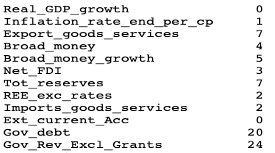
\includegraphics[width = 150mm]{immagini/missn.png}
	\caption{Missing Values in the dataset}
	\label{fig:missn}
\end{figure}
This is a challenge in macroeconomic data collection, but it is typical of economies in sub-Saharan Africa, particularly The Gambia. Now this challenge also happens to be our first challenge in this research. There are several techniques for dealing with missing values. Simple techniques like mean, median or linear interpolation techniques could be used to handle missing values. The missing values could also be dropped if the amount of missing data is too small to affect the total data set. It would be naïve if we decided to drop the null values because it will hugely reduce the data we have. Our choice of methods to fill these missing values would also affect the performance of the various models we are to implement. Therefore, we decided to do away with simplistic methods of imputing missing values since our data has a large amount of missing data.

\subsection{IMPUTATION OF MISSING VALUES}
The idea is to apply two different techniques of imputing missing values, then used the final data derived from each of these techniques and feed the data sets to our models. This would help us understand if the techniques applied will affect the accuracy of a model. Since we are applying different classes of forecasting models, it would be wise to consider linear and non-linear techniques of missing data imputations bearing in mind that the missing values are missing at random (MAR).
\begin{enumerate}
	\item Multiple Imputation by Chained Equation (MICE): is a robust, informative method of dealing with missing data in datasets. The procedure imputes missing data in a dataset through an iterative series of predictive models. In each iteration, each specified variable in the dataset is imputed using the other variables in the dataset. It works in stages by performing multiple regressions over random sample of the data, then takes average of the multiple regression values and impute the missing feature value for the data point. The missing values are imputed based on the observed values for a given individual and the relations observed in the data for other participants, assuming the observed variables are included in the imputation model. The approach is very flexible and can handle variables of varying types as well as complexities (J.Azur et al…2011).
	\item Softimpute: Is one of the Iterative methods for matrix completion that use nuclear-norm regularization. It fits a low-rank matrix approximation to a matrix with missing values via nuclear-norm regularization. The algorithm works like Expectation Maximization (EM), filling in the missing values with the current guess, and then solving the optimization problem on the complete matrix using a soft-thresholded SVD. Special sparse-matrix classes available for very large matrices. The EM step extends the algorithm from the SVDImpute method. Softimpute exploits the special "sparse plus low-rank" structure of the matrix iterates to allow efficient SVD in each iteration. It is a state-of-the-art algorithm for matrix completion. At iteration t, let the current iterate be Xt. The missing values in O are filled in as:
\begin{equation}
 Z_t= P_\Omega (O)+ P_\Omega^\bot  (X_t ) = P_\Omega (O-X_t ) + X_t  \, .
	\label{eq:softimpute}
\end{equation}\\
Where $\Omega_{ij}^\bot =1-\Omega_{ij} \textrm{ is the complement of } \Omega$.
	
\end{enumerate}
\section{MODELS}
\begin{enumerate}
	\item Vector Autoregression (VAR) Model: The VAR model is one of the most successful, flexible, and easy to use models for the analysis of multivariate time series. It is a natural extension of the univariate autoregressive model to dynamic multivariate time series. It has proven to be especially useful for describing the dynamic behavior of economic time series and for forecasting. VAR is a multivariate time series model containing a system of n equations of n distinct, stationary response variables as linear functions of lagged responses and other terms. VAR models are also characterized by their degree p; each equation in a VAR(p) model contains p lags of all variables in the system.  
	\begin{equation}
		y_t=c +\delta_t+\beta x_t  +  \sum}^{p}__{j=1} }  \Phi_j y_{t-1} } +   \epsilon_t   .
		\label{eq:VAR}
		\end{equation}
	\begin{itemize}
		\item 	Where \(y_t\) is n-by-1 vector of distinct response time series variables at time t.
		\item 	c is an n-by-1 vector of constant offsets in each equation.
		\item 	\(\Phi_j\)  is an n-by-n matrix of AR coefficients, where j = 1,…p .
		\item 	\(\epsilon_t\) is an n-by-1 vector of random Gaussian innovations, each with a mean of 0 and collectively an n-by-n covariance matrix \(\Sigma\). For t$\neq$ s, \(\epsilon_t\) and \(\epsilon_s\) are independent.
		\item 	\(x_t\) is an m-by-1 vector of values corresponding to m exogenous variables or predictors. In addition to the lagged responses, exogenous variables are unmodeled inputs to the system. Each exogenous variable appears in all response equations by default.
		\item 	\(\beta\) is an n-by-m matrix of regression coefficients. Row j contains the coefficients in the equation of response variable j.
		\item 	\(\delta\) is an n-by-1 vector of linear time-trend values.
		Generally, the time series \(y_t\) and \(x_t\) are observable because you have data representing the series. The values of c, \(\delta\), \(\beta\), and the autoregressive matrices \(phi_j\) are not always known. We typically want to fit these parameters to our data. The implementation of the VAR model requires preliminary tests that need to be conducted to verify if basic assumptions about the model hold with our data set.
		
	\end{itemize}
       \begin{enumerate}   
	\item Granger Causality Test: The basis behind Vector Autoregression is that each of the time series in the system influences each other. We implemented the Granger Causality test to see if this assumption holds for our data set, the results of which shall be discussed in the next chapter. Granger Causality is a statistical concept of causality that is based on prediction. According to Granger causality, if a series \(X_1\) "Granger-causes" a series \(X_2\), then past values of \(X_1\) should contain information that helps predict \(X_2\) above and beyond the information contained in past values of \(X_2\) alone. Its mathematical formulation is based on linear regression modeling of stochastic processes (Granger 1969). More complex extensions to nonlinear cases exist, however these extensions are often more difficult to apply in practice.
	\item Cointegration Test: Cointegration test helps to establish the presence of a statistically significant connection between two or more time series. If two or more series are individually integrated, but some linear combination of them has a lower order of integration, then the series are said to be cointegrated. A common example is where the individual series are first-order integrated (I(1))  but some cointegrating vector of coefficients exists to form a stationary linear combination of them. We conducted this test using the Johanson test, which is a procedure for testing cointegration of several, say k,I(1) time series. This test permits more than one cointegrating relationship but might not perform well on very small sample sizes. Ours is not a large sample size but consist of many predictors and there are subsequent tests that would make sure everything goes well before fitting our model.
	\item Stationarity Test: When implementing a VAR model, it is customary to check all the time series in the system for stationarity. A stationary time series is one whose properties do not depend on the time at which the series is observed. Thus, time series with trends, or with seasonality, are not stationary. The trend and seasonality will affect the value of the time series at different times. A unit root test tests whether a tme series variable is non-stationary and possesses a unit root. The null hypothesis is generally defined as the presence of a unit root and the alternative hypothesis is either stationary, trend stationarity or explosive root depending on the test used. To test for the unit root test, we conducted the popular Augmented Dickey-Fuller (ADF) test. The intuition behind the test is that if the series is characterized by a unit root process, then the lagged level of the series \((y_(t-1))\) will provide no relevant information in predicting the change in \(y_t\)  besides the one obtained in the lagged changes \(({\Delta y}_(t-k))\). In this case the $\gamma$=0 and null hypothesis is not rejected. In contrast, when the process has no unit root, it is stationary and hence exhibits reversion to the mean.  so, the lagged level will provide relevant information in predicting the change of the series and the null of a unit root will be rejected. The ADF test expands the Dickey-Fuller test equation to include high order regressive process in the model.
		\begin{equation}
	{\Delta y}_t= \alpha + \beta_t +{\gamma y}_{t-1} + \delta_1  \Delta y_{t-1 } +\cdots+ \delta_{p-1} \Delta y_{t-p+1} + \epsilon_t  \, .
\label{eq:DF}
\end{equation}
where \(\alpha\) is a constant, \(\beta\) the coefficient on a time trend and p the lag order of the autoregressive process. Imposing the constraints \(\alpha\)=0 and  \(\beta\)=0 corresponds to modelling a random walk and using the constraint  \(\beta\)=0 corresponds to modeling a random walk with a drift.
\\
If for instance the series are not stationary after conducting the ADF test, we can conduct a differencing technique again and again until all our series become stationary. Differencing is a technique used to convert nonstationary time series to stationary time series. Differencing series is the change between consecutive data points in the series.
	\begin{equation}
   y_t {^'} = y_t - y_{t-1}  \, .
 \label{eq:difference}
 \end{equation}
The equation 4 shows a time series and a first order differenced time series.  In some cases, just differencing once will still yield a nonstationary time series. In that case a second order differencing is required. Second order differencing is the change between two consecutive data points in a first order differenced time series. To generalize, differencing of order d is used to convert nonstationary time series to stationary time series. We shall find more details on the number of times we would have differenced our data in the next chapter.
         \end{enumerate}
\item Random Forests (RF) Model: We implemented the RF model as one of the ML models to compare with our benchmark. As we have seen in (Yoon, 2020, Qureshi et al. 2021, Martin, 2019.  etc), RF has high accuracy compared to other ML models and Traditional models. Our main motivation is that the model is known for handling erratic data with missingness. RF is a regression technique that combines the performance of numerous decision trees algorithms to classify or predict the value of a variable.  That is when RF receives an (x) input vector, made up of the values of the different evidential features analyzed for a given training area, RF builds a number K of regression trees and averages the results. After K such trees \({T(x)}_1^K\) are grown, the RF regression predictor is:
	\begin{equation}
	\hat{f}_{rf}^k (x) = \frac{1}{k} \sum^k_{k=1} T(x)  \, .
\label{eq:RF}
\end{equation}
To avoid the correlation of the different trees, RF increases the diversity of the trees by making them grow from different training data subsets created through a procedure called bagging. Bagging is a technique used for training data creation by resampling randomly the original dataset with replacement. i.e., with no deletion of the data selected from the input sample for generating the next subset \({h(x,\Theta_k), k = 1,…,K}\), where \({\Theta_{kk}}\) are independent random vectors with the same distribution. Hence, some data may be used more than once in the training, while others might never be used. Thus, greater stability is achieved, as it makes it more robust when facing slight variations in input data and, at the same time, it increases prediction accuracy. The process of constructing many trees under similar but randomly drawn conditions minimizes model variance while keeping bias uniform. 
\item 	Support Vector Machines (SVM): are supervised learning models with associated learning algorithms that analyze data for classification and regression analysis. Developed by Vladimir Vapnik et al. in the 1990’s, SVMs are one of the most robust prediction methods, being based on statistical learning frameworks. A SVM constructs a hyperplane or set of hyperplanes in a high or infinite-dimensional space, which can be used for classification, regression, or other tasks like outlier detection. Support Vector Regression (SVR) model fits a linear regression on input data that has been mapped using a non-linear function. The non-linear function can take on various functions \(k(x_i,x_j )\), such as a Gaussian radial basis function kernel: 
\begin{equation}
	k(x_i,x_j )=exp(|x_i- x_j |^2)  \, .
	\label{eq:SVM}
\end{equation}
\(k(x_i,x_j )\)  transforms the input variables x into a higher-dimensional space to better model patterns in the data. The linear regression yields a hyperplane in which each \(y_i\) resides within a hard margin of error \(\epsilon: (\hat{y}_i -\epsilon) \leq y \leq (\hat{y}_i +\epsilon)\). Each prediction \(\hat{y}_i\) is found on this hyperplane. This constrained optimization problem can be infeasible as some observations may lie beyond the margin, thus a cost parameter C can “soften” the margins. A soft margin of error allows some observations to reside beyond the margin but penalizes those observations by their distance from the margin, thereby regularizing the model to reduce the incidence of overfitting. SVR may require more time to train than other algorithms, thus for cost efficiency (C. Chen et al. 2019).
\item 	Elastic Net: The elastic net (Zou and Hastie, 2005) penalty attempts to combine to advantages of both ridge regression and LASSO, namely shrinkage and sparsity together. It is a regularized regression method that linearly combines the \(L_1\) and \(L_2\) penalties of the LASSO and ridge methods. This combination allows for a model to not be too dependent on the selection made by LASSO, yet allow for model interpretability by limiting the number of variables from a large predictor space. This is done by minimizing the sum of squared residual (RSS) subject to both ridge and LASSO penalties as shown below (Kar et al. 2021):
\begin{equation}
   \beta_{\hat{elastic net}} = \underset{\beta}{argmin} \Bigg\{ \sum^N_{i=1} (y_i \beta_o - \sum^p_{p=1} \beta_p x_{pi})^2 + \lambda \sum^p_{p=1} (\alpha |\beta_p| + (1- \alpha) \beta_{p^2})\Bigg\}   \, .
	\label{eq:EN}
\end{equation}
Here, we have two hyperparameters $\lambda$ and $\alpha$. $\lambda$, as before, ranges from 0 to infinity and increases the degree to which parameter estimates are shrunk. $\alpha$, the new hyperparameter, determines the relative importance of the LASSO and ridge penalties. It ranges from 0 to 1. If $\alpha$ = 0, then the LASSO penalty drops out and we have a ridge regression. If $\alpha$ = 1, the ridge penalty drops out and we have a LASSO formulation. This combination allows for relatively stable coefficients (with low variance) in the presence of “Fat” data and multicollinearity. The elastic net method improves lasso’s limitations, i.e., where lasso takes a few samples for high dimensional data. Its net procedure provides the inclusion of N number of variables until saturation. If the variables are highly correlated groups, lasso tends to choose one variable from such groups and ignore the rest entirely.

\item Long Short-Term Memory (LSTM): We use LSTM as an alternative model in our experiment because these networks are well-suited to classifying, processing and making predictions based on time series data, since there can be lags of unknown duration between important events in a time series. LSTM is a special kind of Recurrent Neural Network (RNN) with additional features to memorize the sequence of data. The memorization of the earlier trend of the data is possible through some gates along with a memory line incorporated in a typical LSTM. Each LSTM is a set of cells, or system modules, where the data streams are captured and stored. The cells resemble a transport line (the upper line in each cell) that connects out of one module to another one conveying data from past and gathering them for the present one. Due to the use of some gates in each cell, data in each cell can be disposed, filtered, or added for the next cells. Hence, the gates, which are based on sigmoidal neural network layer, enable the cells to optionally let data pass through or disposed. RNN is a special case of neural network where the objective is to predict the next step in the sequence of observations with respect to the previous steps observed in the sequence. In fact, the idea behind RNN is to make use of sequential observations and learn from the earlier stages to forecast future trends. They were introduced by Hochreiter \& Schmidhuber (1997) and are explicitly designed to avoid the long-term dependency problem. Remembering information for long periods of time is their default behavior, not something they struggle to learn. Each sigmoid layer yields numbers in the range of zero and one, depicting the amount of every segment of data ought to be let through in each cell. More precisely, an estimation of zero value implies that “let nothing pass through”; whereas; an estimation of one indicates that “let everything pass through.” Three types of gates are involved in each LSTM with the goal of controlling the state of each cell (Siami-Namini et al. 2018): 
\begin{itemize}
      \item Forget Gate outputs a number between 0 and 1, where 1 implies “completely keep this”; whereas 0 implies “completely ignore this”.
      \item Memory Gate chooses which new data need to be stored in the cell. First, a sigmoid layer, called the “input door layer” chooses which values will be modified. Next, a tanh layer makes a vector of new candidate values that could be added to the state. 
      \item Output Gate decides what will be yielded out of each cell. The yielded value will be based on the cell state along with the filtered and newly added data.
     \end{itemize}
    
\end{enumerate}
\section{MODEL EVALUATION}
We implemented two evaluation matrices to test and compare the performances of each of the models used in this research.
\begin{enumerate}
	\item Root Mean Squared Error (RMSE): is a measure frequently used for assessing the accuracy of prediction obtained by a model. RMSE measures the differences or residuals between actual and predicated values. It represents the square root of the second sample moment of the differences between predicted values and observed values or the quadratic mean of these differences. The metric compares prediction errors of different models for a particular data and not between datasets. The formula for computing RMSE is as follows: 
	\begin{equation}
		RMSE= \sqrt{\frac{1}{N}\sum^N_{i=1} (\hat{x}_i - x_i)^2}  \, .
		\label{eq:RMSE}
	\end{equation}
	Where N is the total number of observations, \(x_i\)  is the actual value, whereas \(\hat{x}_i\) is the predicated value. The main benefit of using RMSE is that it penalizes large errors. 
	\item 	Mean Absolute Error (MAE): The MAE is one of the several ways of comparing forecasts with their eventual outcomes. It is simply the average absolute vertical or horizontal distance between each point in a scatter plot and the \(\hat{x}_i=x_i\) line. In other words, MAE is the average absolute difference between \(x_i\) and \(\hat{x}_i\). Furthermore, each error contributes to MAE in proportion to the absolute value of the error. This is in contrast with RMSE which involves squaring the differences, so that a few large differences will increase the RMSE to a greater degree than the MAE:
	\begin{equation}
		MAE= \sqrt{\frac{1}{N}\sum^N_{i=1} |\hat{x}_i - x_i|}  \, .
		\label{eq:MAE}
	\end{equation}
\end{enumerate}
\section{SHAPLEY VALUES}
 Since ML models have been criticked as “black-box” models because of their complexities in interpretability, researchers have very recently started to explore ways of interpreting and extracting individual attribute contribution to the prediction of an ML model. Originally, Shapley values were introduced in game theory (Shapley L. 1953) as a way to determine the contribution of individual players in a cooperative game. Shapely values estimate the increase in the collective pay-off when a player joins all possible coalitions with other players. They provide a solution to the assignment of a fair or reasonable reward to each player and represent a unique result characterized by the natural properties or axioms of local accuracy (additivity), consistency (symmetry), and nonexistence (null effect). Strumbelj and Kononenko (2010) used this approach to estimate the contribution of variables to a model prediction, where the variables and the predicted value are analogous to the players and payoff in a game:
 	\begin{equation}
 	\phi^s_k (\hat{f}, x) = \sum_{x^'} \leq C(x)\setminus{k} }  \frac{|x'|! (n - |x'| - 1)}{n!} [\hat{f} (x' \cup \{k\}) - \hat{f} (x')] 
 	\label{eq:SHAP}
 \end{equation}
 where \(C(x)\setminus{k}\) is the set of all possible coalitions of m - 1 model variables when excluding the $\((k^{th})\)$ variable. \(|x^'}|\) denotes the number of included variables. The equation above is the weighted sum of marginal contributions of variable k accounting for the number of possible coalitions for a certain \(x^'\). Intuitively, the above definition of a Shapley value is similar to the regression anatomy of a coefficient $\(\hat{\beta}_k$ , i.e. the bivariate slope coefficient after partialling out all other regressors in a multi-variate model. 
To assess the significance of individual variable contributions, one can reformulate an inference problem in terms of a model’s Shapley decomposition. That is, one estimates the Shapley regression.
	\begin{equation}
	y_i = \Phi^s_i \hat{\beta}^s + \hat{\epsilon}_i= \sum^m_k \phi^s_k (\hat{f}, x_i) \hat{\beta}^s_k \hat{\epsilon}_i  
\label{eq:shap_reg}
\end{equation}
where k = 0 corresponds to the intercept and \(\hat{\epsilon}_i  ~ N(0,\sigma^2_\epsilon)\). The surrogate coefficients \(\hat{\beta}_k^s\) are tested against the null hypothesis.
	\begin{equation}
	H^k_0 (\Omega)  \colon \{\beta^s_k \leq 0 | \Omega\} \, 
	\label{eq:hyp}
\end{equation}
The key difference to the linear case is the regional dependence on \(\Omega\), i.e. only local statements about the significance of variable contributions can be made. This is related to the potential non-linearity of a model whose hyperplane in the input-target space may be curved compared to that of the linear model.
\\
Besides its consistency, our motivation to use the Shapley value framework is derived from Buckmann et al. (2021), where they use it show the significance of predictors in the ML models and compared it with the linear models.

%			CAPITOLO 5: Test
% 

\chapter{RESULTS AND ANALYSIS}
\label{cap5}
\section{Model Implementation}
\begin{enumerate}
	\item VAR: The VAR model was implemented using the “statsmodels” library in python. It has several functions that would easily implement our task at hand.
\\
	First, as we have mentioned in chapter 4, we tested for causality using the Granger causality test. This is one of the prerequisites for implementing a VAR model. Remember after the imputation of our missing values, we now have two different data sets. The one generated from the softimpute imputation and that which was generated from the MICE method. For the softimpute data, the result shows that all our variables have a causation except for \textit{Tot\_reserves} and \textit{Broad\_money\_growth}, \textit{Export\_goods\_services} and \textit{Broad\_money\_growth}, \textit{Export\_goods\_services} and \textit{Tot\_reserves}, \textit{Broad\_money} and \textit{Inflation\_rate\_end\_per\_cp}, and \textit{Imports\_goods\_services}; all with a p-value more than the significance level threshold. The Granger Causality test require that all the variables appear in the form of a matrix where a variable appears both as a dependent and an independent variable. In that case, some variables may have a reverse causality whilst some may not. In our case, it is only \textit{Export\_goods\_services} and \textit{Tot\_reserves} that failed to have a causation in both cases. i.e taking either of the variables as independent or dependent. When the same test was conducted on the MICE data, the result is somewhat different with the softimpute data. Apart from \textit{Inflation\_rate\_end\_per\_cp} and \textit{Export\_goods\_services}, and \textit{Inflation\_rate\_end\_per\_cp} and \textit{Tot\_reserves}, there is a causation in every other comparison. Even with the two cases that failed, this also is just a one-way causation failure. i.e causation failed only in the case when \textit{Inflation\_rate\_end\_per\_cp} was the dependent variable.
\\
	For the Cointegration Test, we conducted the Johanson test on both of our data sets. There is a cointegration with a variable and all other variables if the test statistics is less than the critical value (95\% confidence interval). On the softimpute data, it is only \textit{Real\_GDP\_growth} that has its test statistics less than the critical value. This means that there is a connection between  \textit{Real\_GDP\_growth} and all other variables. This would not cause us problems since it is our main variable of interest. On the MICE data, again there has been a little difference on the result. The cointegration test was true on Real GDP growth, Export of Goods and Services, and \textit{Inflation Rate end of period consumer price}. They all have a test statistic less than the respective critical values.
\\
	Before going any further, at this stage, we split our data in to training and test sets. The training set represents 80 percent of the data whilst the test set represents 20 percent, making it 38 and 8 observations respectively. 
\\
	We remember that ADF test was conducted in chapter 4 to test for seasonality in our data. We found out that only two out of twelve variables (series) in the softmax data were stationary whilst three were stationary in the MICE data. The idea now is to make all those non-stationary variables stationary by applying the traditional differencing method. After applying the first differencing stage on our two data, all the variables that were non-stationary became stationary when next ADF was conducted. The forecast values therefore have to be inverted to the original scale of the data since differencing changes the scale of the data.
\\
	Finally, our data is now ready to be fed on to the VAR model for forecasting. However, since the optimal number of lags have to be determined before fitting the model, we applied the information criteria methods for determining the optimal lags for our model. This was more of an automatic process since the size of our data is small, only one lag seems more optimal for the model fitting.
	\item ML Models: The ML models all have somewhat similar data preparation and parameter setting techniques, except for the LSTM model. These models were implemented using two standard modules in Python namely, TensorFlow and Sklearn. The difference with the VAR as regards the data splitting is that for the ML models, we have to set our target variable as well as the predictors. The original training and test sets from the preparations leading to the VAR mode fitting were adopted. We have only detached \textit{Real GDP growth} from both the training set and test set as our target variable (Y\_train and Y\_test respectively). 
\\
	For the RF model, setting up optimal parameters contributes to the performance of the model. One of the key parameters is number of trees to be assigned to the model. We were better off leaving the number of trees at default than when we tried to assign it. The maximum depth of each tree in the forest was set at 4. For the SVM, the regularization parameter is inversely proportional to C which is set at 100.  The EN has what is known as mixing parameters as the key parameters to note. These are the L1 and L2 penalties and L1 is set to equal to 0.9 in the model. The LSTM model is the only model implemented using TensorFlow through which a simple model was built. Before that, we created a function to reshape the structure of our data. This will create windows of data that will be fed into the datasets, for each timestamp T we will append the data from T-7 to T to the X data with target Y(t). With this, the dataset length will be reduced to guarantee all samples have the window and then later joined back since we were sliding. After all we verified to check if both the training and the test data are the same with our previous. The batch size, buffer size and window length were set at 64, 100 and 24 respectively. We choose 'rmsprop' as the optimizer with a dropout of 0.1 and 10 epochs with MAE as the loss function.
	\end{enumerate}
\section{Results}
\begin{enumerate}
	\item Forecast Values:
	From Table 1, the VAR model has provided two different forecasts based on the two types of data sets fed on to the model.  There are some notable forecast values in the table, especially where there is a huge difference between the actual and the forecast values of both data sets. Let us quickly note that the actual value for the year 2022 is a predicted value from the IMF’s projections since the actual figures are release at the end of the year, we took it as an input for our model. This is actually a year after the outbreak of the novel Covid-19 that has rampage the world’s economies. Our model has predicted a slow growth with the Softimpute data and a decline in “Real GDP growth” with the MICE data. The year 2016 was a year when the country experienced a very tense election that almost turned the country in to war. Our forecast values for this year on both data sets are very close with the actual values. This followed a year that saw the country had a new president after more than two decades. There were high expectations, and most people anticipated a booming economy after the country had lost a lot in the tourism sector as well as an increased in the consumer price due to the political impasse. Our model predicted a very high growth in Real GDP on both data sets in that very year. 
	For the ML models, only RF and EN were fed with the two different data generated from the two techniques used for the imputation of missing values. This was enough to do a comparison with the VAR model.
	        \begin{table}
	        	\centering
	        	\begin{tabular}{|l|l|l|l|}
	        		\hline
	        		Year & SoftImpute data & MICE data &  Actual \\ \hline
	        		2015 &   -2.67               &  -0.81                  & 4.10     \\
	        		2016 &   -2.18                     & 1.07                &  1.90     \\
	        		2017 &     6.98             &        8.10                 &  4.8       \\ 
	        		2018  &   2.04                      & 1.77                 &   7.20      \\
	        		2019   &  -3.00                      & -1.64              &  6.10          \\
	        		2020   & -0.65                         & -0.05            &  0.00         \\
	        		2021  &    3.03                       &     5.32             & 6.00           \\
	        		2022 &     1.12                     &       -0.70            &   6.50         \\ \hline
	        	\end{tabular}
	        	\caption{VAR Model Forecasts.}
	        	\label{tab:VAR}
	        \end{table}
	        
	 \begin{table}
		\centering
		\begin{tabular}{|l|l|l|l|l|l|}
			\hline
			Year &\multicolumn{2}{c|}{RF  MODEL}& \multicolumn{2}{c|}{EN MODEL} &  Actual \\ \hline
			          & SoftImpute & MICE       &   SoftImpute &    MICE  &                 \\ 
			2015 &   3.43           & 2.11         & 2.86               &   1.94    & 4.10        \\
			2016 &   3.15            & 1.68         &  0.89              & -1.66    & 1.90        \\
			2017 &     1.60            & 1.56         &  -0.66            &  -1.06  & 4.80       \\ 
			2018  &    1.30            & 1.30          &   -1.15           &  1.78     & 7.20      \\
			2019   &  2.63             & -1.63          & 3.59            &  -1.10   &  6.10          \\
			2020   &  2.50              & 2.60           & 3.24            &  0.26    & 0.00         \\
			2021  &    4.08              &  1.46            & 3.94          &  1.61      & 6.00           \\
			2022 &     3.76               & 1.46             &  2.94         &  1.60      &  6.50         \\ \hline
		\end{tabular}
		\caption{RF \& EN Model forecast.}
		\label{tab: RF_EN}
	\end{table}
		Table 2 shows somewhat interesting results compared to what we saw in Table 1. In 2017, the RF model forecasted a slow growth on both the Softimpute and MICE data whilst the EN model forecasted a decline in growth for both data in the same year. This is in contrast with the VAR model which predicted a high growth that year. However, both the RF and EN models have forecast values showing a slow growth with both data in 2022. These results are similar with that of the VAR model in the same year. We know it is too premature to conclude which models provide better prediction at this point, we would see later in the forecasts’ errors. We can see in both Table 1 and Table 2 the huge differences between the forecast values and the actual values in both models for the period 2018 and 2019. In Table 2, the RF model predicted a slow growth in 2018 and an increase in 2019 for both data. The EN predicted a deeper decline with the Softimpute data and an increase with the MICE data in 2018, and larger increase with the softimpute data in 2019, but a decline in growth with the MICE data in the same period. This was not the case for the VAR model in 2019 as we have seen in Table 1. The model predicted a deeper decline in growth with Softimpute data and a slight decline with the MICE data. This particular period is when the economy of The Gambia started to recover from the 2016 political impasse. The number of tourists inflow reached its peak and there had been an improved sound economic policies with a much freer market system.\\
		  \begin{table}
		 	\centering
		 	\begin{tabular}{|l|l|l|l|}
		 		\hline
		 		MODEL & SoftImpute data & MICE data \\ \hline
		 		RMSE &    5.18              &  4.71      \\
		 		MAE &     4.53               & 3.77       \\  \hline
		 	\end{tabular}
		 	\caption{VAR SoftImpute vs Mice Accuracy.}
		 	\label{tab: VAR_soft_mice}
		 \end{table}
		From Table 3, we can clearly see that the methods we choose to impute the missing values greatly have an impact in the accuracy of the VAR model. The MICE data has better accuracy in both the RMSE and MAE matrices, that is to say that the Softimpute data has higher errors than the MICE data. Let us recall from chapter 4 that the MICE method of missing values imputation is linear in nature whilst the Softimpute method is nonlinear. This suggests that linear methods of missing value imputation could work better with linear or traditional models than with nonlinear models or ML models and vice-versa. We could make that conclusion once we compare the same analogy with our ML models.\\
		Table 4 shows the accuracy of the two ML models used to make an alternative test on the suggestion made earlier about the Softimpute and MICE methods for the imputation of missing values. The forecasting accuracy of both the RF and EN models deteriorated when fed with the MICE data. This is true for both the RMSE and MAE measures. For the RF model, the RMSE increased by 0.68 whilst the MAE increased by 0.66 when comparing the Softimpute and MICE data respectively. The EN model has a difference of 0.29 for the RMSE and 0.52 for the MAE of the two data. This additional finding has provided us with more grounds to say that missing values imputation methods have an impact on the model forecasting accuracy. The true performance of a model would be minimized when fed with data whose missing values were imputed using methods of a different class. We have seen that the data whose missing values were imputed with the MICE data did not perform well with ML models as compared to the VAR model, and the data whose missing values were imputed using the softimpute method did not perform well with the VAR model as compared to the ML models. This finding provides a ground to conclude that linear methods should be chosen to impute missing values of a time series data set with massive missingness if the predicting model to be implemented is linear. A nonlinear method should be applied for imputing the missing values when implementing nonlinear models. We limit this conclusion to the case when there is massive missingness in the data as it is in our case.
		 \begin{table}
			\centering
			\begin{tabular}{|l|l|l|l|l|}
				\hline
				Accuracy &\multicolumn{2}{c|}{SoftImpute data } &\multicolumn{2}{c|}{MICE data } \\ \hline
				&   RMSE & MAE               & RMSE & MAE \\
				RF             &    3.10              &  2.71    &  3.78   &  3.37 \\
				EN             &     4.12              & 3.43   &  4.41    & 3.95 \\  \hline
			\end{tabular}
			\caption{RF \& EN; SoftImpute vs MICE accuracy.}
			\label{tab:RF_EN_soft_mice}
		\end{table}
		
		Now we are ready to show the comparison of the overall performance of each of the models implemented in this research. This would help us make the conclusion as to which models provide the best forecasting accuracy.\\
		 \begin{table}
			\centering
			\begin{tabular}{|l|l|l|l|l|}
				\hline
				Accuracy &\multicolumn{2}{c|}{SoftImpute data } &\multicolumn{2}{c|}{MICE data } \\ \hline
				&   RMSE &         MAE      & RMSE & MAE \\
				VAR           &    5.18            &   4.73    &   4.71  &3.77  \\
				RF             &    3.10              &  2.71    &  3.78   &  3.37 \\
				EN             &     4.12              & 3.43   &  4.41    & 3.95 \\ 
				SVM          &       3.43            & 3.26    &     -         &   -       \\
				LSTM         &       5.44           &  4.91        &    -           &     -      \\ \hline
			\end{tabular}
			\caption{Forecasting errors for all Models.}
			\label{tab:all_MODELS}
		\end{table}
		Finally, Table 5 presents the accuracy of all the models implemented in this research. For the Softimpute data, under the RMSE, the VAR model from the traditional class performs better than the LSTM model but worse than the other three models. However, when we compare the models based on the MAE, the VAR model’s accuracy is just slightly better than the LSTM. The RF model provides the best performance based on the RMSE under the softimpute data and also outperformed all the models when they are compared under the MAE. We remember that the MICE was not fitted with SVM and LSTM, this is why there are blank entries under MICE section of these models. For the MICE data, the VAR model is slightly worse than the EN model under RMSE. The RF model has the best forecasting accuracy under both the MAE and the RMSE for the MICE data. The VAR model has also outperformed the EN model for MAE under the MICE data. Overall, we have seen that the VAR model performed relatively well as compared to the LSTM model under the Softimpute data. This is also the case when the VAR model is compared to the EN model under the MICE data. The performance of the LSTM model could be attributed to the predictive power of such models and that they require relatively large training data. The sample size used in this research is obviously small but has attributes with erratic nature as we can see in Appendix A2, the trend of these attributes over time.
		Even though the VAR model has outperformed LSTM for the RMSE and MAE under Softimpute, and the EN model for MAE under MICE data, there are no huge difference in the errors for both the cases where VAR outperformed and where the said models outperformed it.
		\item Shapley Values for Causal Inference:
		Shapley values allow us to assess the marginal effect of model variables on the predicted outcome. To implement it, we used the SHAP library in python which has functions that can decompose Shapley values from a ML model. The first task is to extract the Shapley values, then we can see the individual variable contributions through the local Force plot. We decided to execute it only on the RF model just to provide us with the requisite information to conclude on our research, but it can be applied on all our ML models.\\
		Figure 2 represents the Shapley values of the RF model where the contribution of each attribute on the prediction of the output is shown. The output of the prediction is 3.43 and the base value is 2.859. The base value technically represents the intercept of the model. If all the predictors are equal to zero, the base value is the expected output of the model. In red, are all the predictors that have a positive impact on the prediction of the output. In other words, an increase in those predictors would result to an increase in Real GDP growth. On the other hand, those predictors in blue have an inverse contribution to the predicted output. An increase in those variables would result to an increase in Real GDP growth. The size of those colored rectangles also signifies the size of the impact of the corresponding predictor on the dependent variable. For example, on the predictors in red, \textit{Net\_FDI} has the highest positive contribution on the prediction of Real GDP growth, followed by \textit{Broad\_money\_growth}. On the predictors in blue, \textit{Ext\_current\_Acc} has the highest inverse contribution on the prediction of Real GDP growth, followed by \textit{REE\_exc\_rates}.
		\begin{figure}[t]
			\centering
			\includegraphics[width = 150mm]{immagini/Shap.png}
			\caption{SHAP Force plot for RF Model}
			\label{fig:SHAP}
		\end{figure}
	One of the key criticisms that the Shapley method of explaining ML model has had is that they may produce non-intuitive results. For example, in Economics, the Shapley estimates could defy fundamental theories about relations among variables. Let’s for example take \textit{Inflation\_rate\_end\_per\_cp} from Figure 2, it has it that an increase in inflation contributes to an increase in Real GDP growth. We know from Economic theory that due to inflation; GDP increases and does not actually reflect the true growth in an economy. That is why Real GDP growth should decrease since the GDP must be divided by the inflation rate (raised to the power of units of time in which the rate is measured) to get the growth of the real GDP. There are reasons why an increase in inflation leads to an increase in GDP, but we would not go into those details in this research. We can use the SHAP feature importance to know the importance of each feature in making the estimates seeing in Figure 2.\\
		Figure 3 shows the importance of the features based on magnitude of feature attributions. From Figure 2, we could recall the impact of the attributes on the prediction output. Figure 3 will then help us understand the importance of each of these attributes in making those estimates. In other words, it shows the significance of the Shapley values of the various attributes. We can see that \textit{Broad\_money} is the most significant predictor since it provides close to 70\% impact on Real GDP growth. This is followed by \textit{Gov\_debt} which provides about 40\% impact. Interestingly, \textit{Inflation\_rate\_end\_per\_cp} whose impact we have queried in Figure 2, has the least importance among all the predictors in our model. In fact, we can conclude that it’s impact on Real GDP growth seen in Figure 2 is insignificant. This is backed by the fact that it provides a significance level close to 0\%.\\
		\begin{figure}[t]
		\centering
		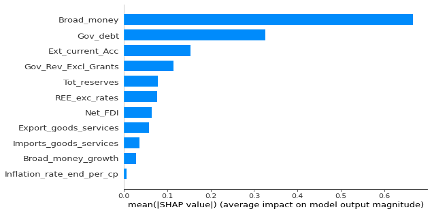
\includegraphics[width = 150mm]{immagini/fea.png}
		\caption{Feature Importance}
		\label{fig:feat}
			\end{figure}
		In traditional econometric models, we have ways to see if there is a non-linear impact between a certain predictor and the target variable. That is to say that the impact of the predictor on the dependent variable has a turning point. We can use a similar approach to see impact of fractures is distributed between lower values and higher values of a particular feature. We would be able to obtain the exact turning point, but we could provide a similar intuition. For that, we shall use the SHAP summary plot to illustrate.
		\begin{figure}[t]
		\centering
		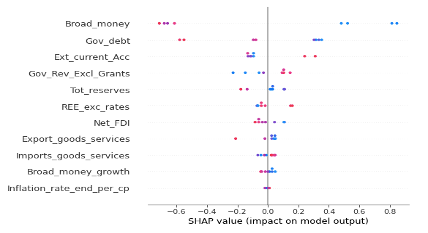
\includegraphics[width = 150mm]{immagini/shapsum.png}
		\caption{SHAP summary plot}
		\label{fig: summary}
	\end{figure}
	 The summary plot in Figure 4 combines feature importance with feature effects. Each point on the summary plot is a Shapley value for a feature and an instance. The colors in the Figure are self-explanatory. They represent the value of the feature from low to high. Overlapping points are jittered in y-axis direction, so we get a sense of the distribution of the Shapley values per feature. Lower values of \textit{Broad\_money} contribute to the prediction of high output whereas very high values of it contribute to the prediction of lower output. In essence, we can say that the impact of Broad money on Real GDP growth has a turning point. An increase in Broad money would increase Real GDP growth up to a certain point, then Real GDP growth will begin to decrease as Broad money increases. The same intuition could be derived from the \textit{Gov\_debt}, only medium and higher values of Government debt have an inverse impact on Real GDP growth. Just as we have seen on the previous Figures, \textit{Inflation\_rate\_end\_per\_cp} again entails results which further ferments our suggestion that its contribution to the model prediction is insignificant. The Shapley values are overlapped exactly on the y-axis cutting at 0 on the x-axis. This presents an ambiguity in understanding what the results really entails. So we can still hold on to the argument of the insignificance of the variable. A similar story could be derived from \textit{Broad\_money\_growth}, but the difference is that we can not make the same conclusion as with \textit{Inflation\_rate\_end\_per\_cp}.  \textit{Broad\_money\_gowth} has visible difference in the colors of the value points, but even in Figure 4, it has the least significance level after \textit{Inflation\_rate\_end\_per\_cp}. 
	\end{enumerate}
		
% 
%			CAPITOLO 6: Conclusioni e sviluppi futuri
% 

\chapter{CONCLUSION}
\label{cap6}

For the past few decades, the macroeconomic forecasting community has witnessed an increase in the body of literature in the use of ML models for forecasting. Many researchers began to explore and compare the performances of these models and the conventional models of time series forecasting in terms of their accuracy.
\\
In this paper, we have compared the performance of traditional models to that of ML models by forecasting the Real GDP growth of the Gambia. The data we used has a large number of missing values, so we implemented two types of missing values imputation techniques and then fed the data generated from each of the two techniques to our various model. We found out that the methods used for the imputation of missing values had an effect on the forecasting accuracy of the applied models. The data generated through the MICE technique has had a positive impact on the VAR model whereas the data generated from the SoftImpute technique had a positive impact on the ML models. In other words, the VAR model provides the best accuracy under MICE than under Softimpute and the ML models performed better under Softimpute than under MICE. We have further seen that the data whose missing values were imputed with the MICE method did not perform well with ML models as compared to the VAR model, and the data whose missing values were imputed using the softimpute method did not perform well with the VAR model as compared to the ML models. Therefore, for the case of massive missingness in data, we conclude that linear methods should be chosen to impute missing values of a time series data set with massive missingness if the predicting model to be implemented is linear. A nonlinear method should be applied for imputing the missing values when implementing nonlinear models.
\\
Overall, ML models can outperform traditional models in forecasting Real GDP growth, especially with data with massive missingness. However, models like LSTM and EN models were outperformed by the benchmark model in some cases. The performance of the LSTM model could be attributed to the predictive power of such models and that they require relatively large training data. The sample size used in this research is obviously small but has attributes with erratic nature as we have seen in the trend of these attributes over time. Although the VAR model has outperformed LSTM and the EN model at some point, but there is no significant difference in both the cases where VAR outperformed these models and where the said models outperformed it.
\\
For conducting inferential analysis using ML, this research implemented the Shapley values method to answer critical questions asked in the beginning. The method was only implemented on the RF model. We found out that \textit{Net\_FDI} has the highest positive contribution on the prediction of Real GDP growth, followed by \textit{Broad\_money\_growth}. \textit{Exc\_current\_Acc} has the highest inverse contribution on the prediction of Real GDP growth, followed by \textit{Real\_exc\_rates}. On the importance of each predictor, we have seen that \textit{Broad\_money} is the most significant predictor since it provides close to 70\% impact on Real GDP growth. This is followed by \textit{Gov\_debt} which provides about 40\% impact. The method showed that \textit{Inflation\_rate\_end\_per\_cp} is not significant in predicting Real GDP growth. The Shapley values method also shows the stages at which each feature contributed to the prediction of the model output, which we contrasted to the turning point phenomenon in econometrics. We have seen that lower values of \textit{Broad\_money} contribute to the prediction of high output whereas very high values of it contribute to the prediction of lower output. In essence, we can say that the impact of Broad money on Real GDP growth has a turning point. An increase in Broad money would increase Real GDP growth up to a certain point, then Real GDP growth will begin to decrease as Broad money increases. The same intuition could be derived from the \textit{Gov\_debt}, only medium and higher values of Government debt have an inverse impact on Real GDP growth.
In conclusion, this paper finds that ML models can outperform traditional models in forecasting Real GDP growth in low-income economies. Methods chosen for imputing missing values can influence the performance of a model if the data suffers a massive missingness. Shapley values provides an interesting explanation of ML models and provides intuitively sound causal inference but might inflate actual relations since the framework is conducted on a model that has already been run.



% 
%			APENDICE: materiali aggiuntivi e dimostrazioni
% 

\appendix

\chapter{DATA}
Figure 5 shows the correlation between all the attributes in our data set. Real GDP growth does not have a strong correlation with all other variables as we can see that the highest correlation is captured with Broad money growth where the correlation is equal to 0.19. This correlation diagram has been developed from the original data with missing values before imputing those missing values. We later constructed another heatmap after imputing the missing values, but there is no significant difference when compared to Figure 5. Other notable correlations amongst our predictors are the correlation coefficients of Export of goods and services and Total reserves, and Broad money and Government revenue excluding grants whose coefficients are equal to 1 and 0.9 respectively. These strong correlations do not cause problems since we do not have such assumptions as prerequisites for the models applied in this research.\\
	\begin{figure}[t]
	\centering
	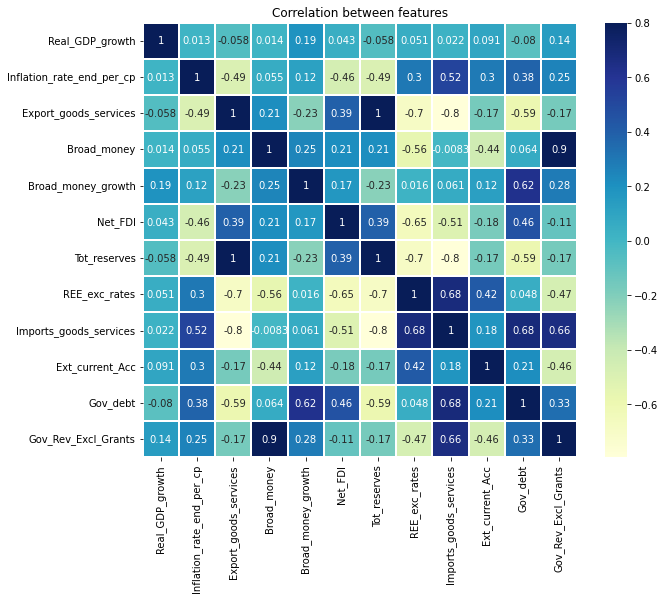
\includegraphics[width = 145mm]{immagini/corr.png}
	\caption{Correlation between Variables}
	\label{fig: corr}
\end{figure}
Figure 6 shows the trend of each variable against year from 1980 to 2022. Real GDP growth has its peak in 1982 when the growth rate was above 20 but fell below 10 in the years to follow. Real effective exchange rate has a unique trend from all the other variables, it started at a high rate in 1980 and had since then fluctuated in a decreasing rate until 2022. Inflation has its highest rate in 1986 and has since then fallen below 20 in the years after. Except for Real GDP growth, all other variables dropped in 2022 form the preceding year. We recall that the estimates for 2022 were projected estimates by IMF which we took as our inputs and those variables without an instance in that year were consider as missing and imputed through the missing values imputation methods we applied as explain in chapter 4. Figure 6 was plot from the data generated from the application of the Softimpute method.\\
	\begin{figure}[t]
	\centering
	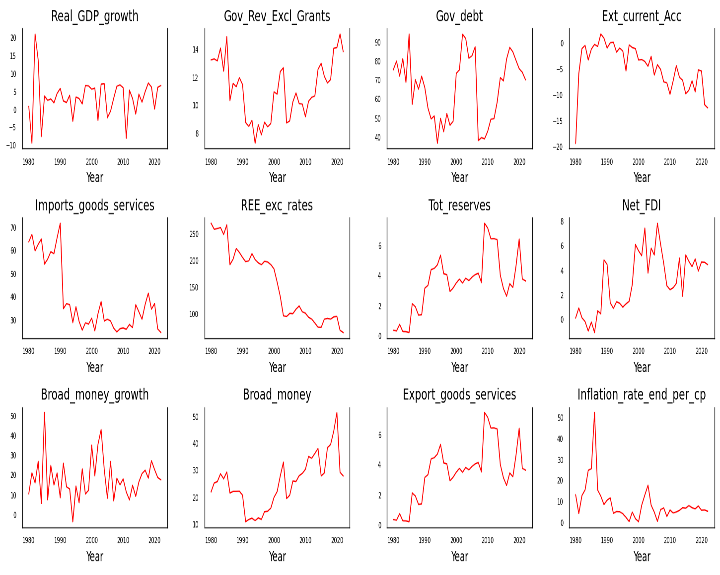
\includegraphics[width = 145mm]{immagini/trend.png}
	\caption{Trend of Series}
	\label{fig:trend}
\end{figure}

\chapter{MODEL RESULTS PLOT}
	\begin{figure}[t]
	\centering
	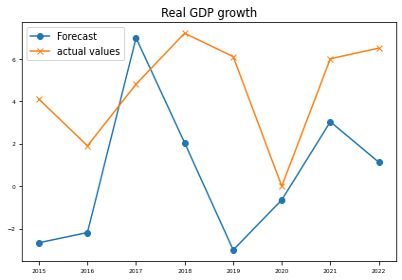
\includegraphics[width = 130mm]{immagini/vfor.png}
	\caption{VAR Forecast for SoftImpute}
	\label{fig:var_forcast}
\end{figure}
Figure 7 shows the plot generated from estimates of the VAR model through the data generated from the Softimpute imputation method. The errors made by the error in forecasting the instance of the Real GDP growth in each considered year, are obvious in the graph. The model forecasted a contraction in the economy in 2015, 2016 and 2019, when the actual growth rates are above 2. There are bigger errors in 2015 and 2019 than in 20016. The smallest forecast errors of the VAR model can be spotted in 2017 and 2020. In fact, in 2017, the model forecasted a growth rate higher than the actual rate. We could recall from our explanation in chapter 5, that 2017 was when the experience a change of government after more than two decades and the economy had started to recover from 2016 when there had been a political impasse that almost saw the country plunge in to war. 2020 has the smallest error as we can see it has the closest distance between the actual rate and the forecast rate. This as we have explained before, is also a year when Covid19 hit the global economy.\\
Figure 8 represents the graph of the forecast made by the VAR model through the data generated by MICE imputation method. It provides better forecast estimates as compared with results generated through the Softimpute method. This was well detailed in chapter 5. In Figure 8 the estimates with the lowest errors are 2020, 2021, 2016 and 2017. The model provides almost a perfect prediction in 2020 and a much smaller in 2021 than in Figure 7. However, in both graphs, 2017 is the only year when the model forecast a rate higher than the actual rate.
\\
\begin{figure}[t]
	\centering
	\includegraphics[width = 130mm]{immagini/vfor1.png}
	\caption{VAR Forecast for MICE}
	\label{fig: var_mice}
\end{figure}

Figure 9 and 10 show the plots of the forecast made by the RF model through data generated by Softimpute and MICE respectively. As we have explained in chapter 5 that our ML models performed better on the Softimpute data than the MICE, this could also be seen on both the Figures 9 and 10. Figure 9 shows lower errors in 2016, 2020 and 2021 whereas 10 shows low errors in 2016 and 2020.\\
\begin{figure}[t]
	\centering
	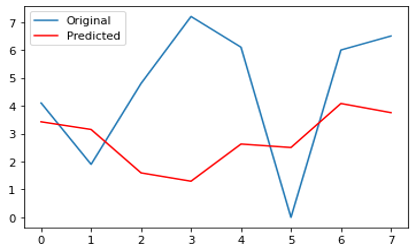
\includegraphics[width = 130mm]{immagini/RF.png}
	\caption{RF Forecast for SoftImpute}
	\label{fig: RF_softimpute}
\end{figure}
\begin{figure}[t]
	\centering
	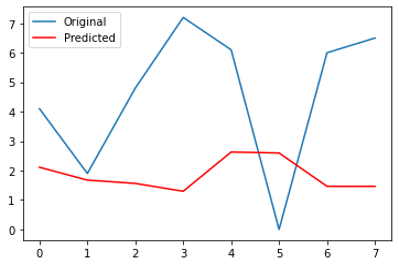
\includegraphics[width = 130mm]{immagini/RF1.png}
	\caption{RF Forecast for MICE}
	\label{fig:RF_MICE}
\end{figure}
Figure 11 and 12 represent plots from the forecast of the EN model generated from the Softimpute and MICE data respectively. We have wider gaps between the forecast values and the actual values in Figure 11 than in Figure 12, except for year 2020 when Figure 12 a gap closer than that of Figure 11.\\
\begin{figure}[t]
	\centering
	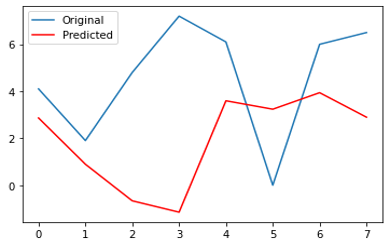
\includegraphics[width = 130mm]{immagini/EN.png}
	\caption{EN Forecast for SoftImpute}
	\label{fig:EN_soft}
\end{figure}
\begin{figure}[t]
	\centering
	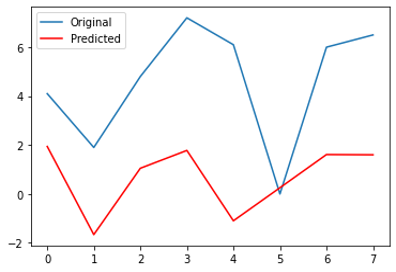
\includegraphics[width = 130mm]{immagini/EN1.png}
	\caption{EN Forecast for MICE}
	\label{fig:EN_MICE}
\end{figure}
Figure 13 and 14 represent the plots of the predictions of LSTM model and SVM model respectively. As we have seen so far, the LSTM model provides the worst forecast errors, at least under the Softimpute data since we did do execute it on the MICE data. Figure 13 shows that the model has only one estimate which is close to the actual value, that is 2021. Most of its forecast value are 0 and below. SVM has two forecast estimates that are closer to the actual values. As we can see on Figure 14, 2016 and 2020 are the years with least forecast errors, 2017 is better than the remaining years.
\begin{figure}[t]
	\centering
	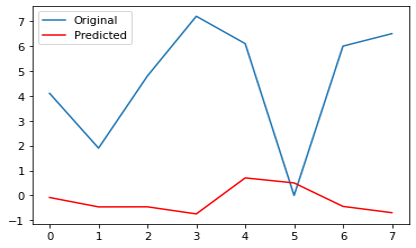
\includegraphics[width = 130mm]{immagini/lstm.png}
	\caption{LSTM Forecast}
	\label{fig:LSTM}
\end{figure}
\begin{figure}[t]
	\centering
	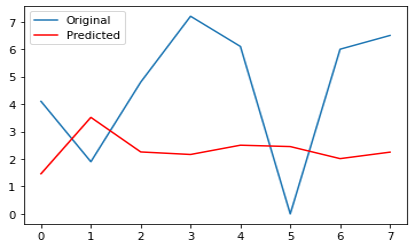
\includegraphics[width = 130mm]{immagini/svm.png}
	\caption{SVM Forecast}
	\label{fig:SVM}
\end{figure}

\chapter{GLOBAL FORCE PLOT OF SHAPLEY VALUES}
\begin{figure}[t]
	\centering
	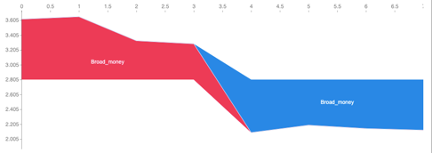
\includegraphics[width = 150mm]{immagini/bm.png}
	%\caption{EN Forecast for MICE}
	%\label{fig:missn.png}
\end{figure}
Unlike Figure 4 from chapter 5, the Figures in Appendix C represent global force plot where the detail contribution of each variable is shown. The contribution of every instance of a feature to the prediction of a model is clearly shown. Just like before the red color indicates the portion of a feature which contributes to the prediction of higher output and the blue color shows the portion that contributes to the lower prediction of the output. 
\begin{figure}[t]
	\centering
	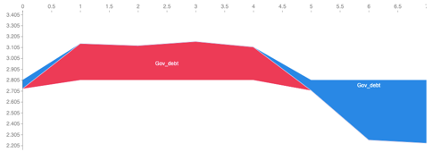
\includegraphics[width = 150mm]{immagini/gd.png}
	%\caption{EN Forecast for MICE}
	%\label{fig:missn.png}
\end{figure}
\begin{figure}[t]
	\centering
	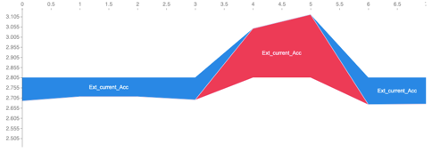
\includegraphics[width = 150mm]{immagini/ext.png}
	%\caption{EN Forecast for MICE}
	%\label{fig:missn.png}
\end{figure}
\begin{figure}[t]
	\centering
	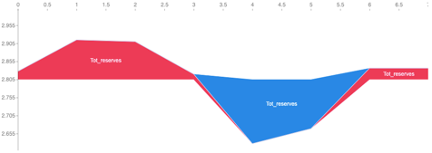
\includegraphics[width = 150mm]{immagini/tr.png}
	%\caption{EN Forecast for MICE}
	%\label{fig:missn.png}
\end{figure}
\begin{figure}[t]
	\centering
	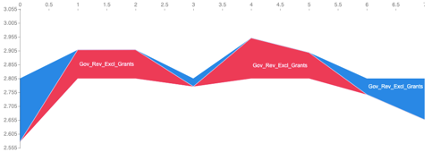
\includegraphics[width = 150mm]{immagini/gr.png}
	%\caption{EN Forecast for MICE}
	%\label{fig:missn.png}
\end{figure}
\begin{figure}[t]
	\centering
	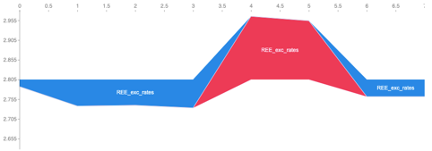
\includegraphics[width = 150mm]{immagini/ree.png}
	%\caption{EN Forecast for MICE}
	%\label{fig:missn.png}
\end{figure}
\begin{figure}[t]
	\centering
	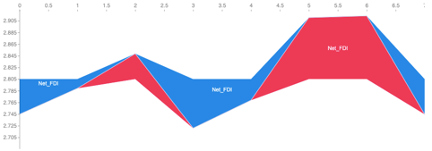
\includegraphics[width = 150mm]{immagini/fdi.png}
	%\caption{EN Forecast for MICE}
	%\label{fig:missn.png}
\end{figure}
\begin{figure}[t]
	\centering
	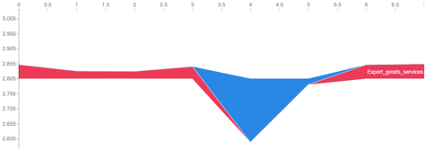
\includegraphics[width = 150mm]{immagini/exp.png}
	%\caption{EN Forecast for MICE}
	%\label{fig:missn.png}
\end{figure}
\begin{figure}[t]
	\centering
	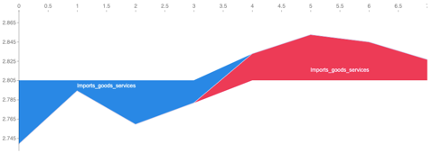
\includegraphics[width = 150mm]{immagini/imp.png}
	%\caption{EN Forecast for MICE}
	%\label{fig:missn.png}
\end{figure}
\begin{figure}[t]
	\centering
	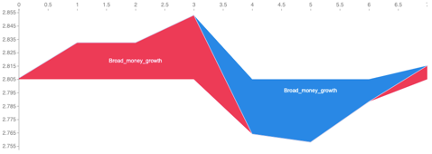
\includegraphics[width = 150mm]{immagini/bmg.png}
	%\caption{EN Forecast for MICE}
	%\label{fig:missn.png}
\end{figure}
\begin{figure}[t]
	\centering
	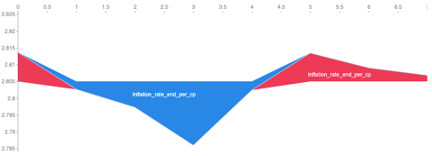
\includegraphics[width = 150mm]{immagini/inf.png}
	%\caption{EN Forecast for MICE}
	%\label{fig:missn.png}
\end{figure}


%
%			BIBLIOGRAFIA
%
\begin{thebibliography}{8}
	\addcontentsline{toc}{chapter}{BIBLIOGRAPHY}
	\bibitem{ref_article1}
Ulke, Volkan and Sahin, Afsin and Subasi, Abdulhamit : A comparison of time series and machine learning models for inflation forecasting: empirical evidence from the US.  Neural Computing and Applications: \textbf1519--1527  (2018)
 \bibitem{ref_book1}
 Basuchoudhary, Atin and Bang, James T and Sen, Tinn: A comparison of time series and machine learning models for inflation forecasting: empirical evidence from the US. Springerr, (2017)
 \bibitem{ref_proc1}
 Buckmann, Marcus and Joseph, Andreas and Robertson, Helena: An interpretable machine learning workflow with an application to economic forecasting, mimeor,  (2021)
	\bibitem{ref_article1}
	Chuku, Chuku and Oduor, Jacob and Simpasa, Anthony : Intelligent forecasting of economic growth for African economies: Artificial neural networks versus time series and structural econometric models, Washington Research Program on Forecasting: \textbf28  (2017)
	\bibitem{ref_article1}
	Cicceri, Giovanni and Inserra, Giuseppe and Limosani, Michele : A machine learning approach to forecast economic recessions—an italian case study.  Multidisciplinary Digital Publishing Institute: \textbf241  (2020)
	\bibitem{ref_article1}
	Coulombe, Philippe Goulet and Marcellino, Massimiliano and Stevanovic, Dalibor : Can machine learning catch the Covid-19 recession?.  Cambridge University Press: \textbf71--109  (2021)
	\bibitem{ref_article1}
	Diebold, Francis X: The past, present, and future of macroeconomic forecasting.  Journal of Economic Perspectives: \textbf175--192 (1998)
	 \bibitem{ref_book1}
	Guegan, Dominique and Rakotomarolahy, Patrick: Alternative methods for forecasting GDP. In Nonlinear Modeling of Economic and Financial Time-Series. Emerald Group Publishing Limited, (2010)
	\bibitem{ref_lncs1}
	Araujo, Gustavo Silva and Gaglianone, Wagner Piazza: Machine learning methods for inflation forecasting in Brazil: New contenders versus classical models. Mimeo , (2020)
	\bibitem{ref_lncs1}
	Tkacz, Greg and Hu, Sarah: Forecasting GDP growth using artificial neural networks. Bank of Canada , (1999)
	 \bibitem{ref_book1}
	Chen, Jeffrey C and Dunn, Abe and Hood, Kyle and Driessen, Alexander and Batch, Andrea: Off to the races: A comparison of machine learning and alternative data for predicting economic indicators. In Big Data for 21st Century Economic Statistics. University of Chicago Press, (2019)
	 \bibitem{ref_book1}
	Jung, Jin-Kyu and Patnam, Manasa and Ter-Martirosyan, Anna: An algorithmic crystal ball: Forecasts-based on machine learning. International Monetary Fund, (2018)
		\bibitem{ref_article1}
Kurihara, Yutaka and Fukushima, Akio and others: AR model or machine learning for forecasting GDP and consumer price for G7 countries.  Redfame publishing: \textbf1 (2019)
	\bibitem{ref_article1}
Syed, Ateeb Akhter Shah and Lee, Kevin Haeseung: Macroeconomic forecasting for Pakistan in a data-rich environment. Taylor \& Francis: \textbf1077--1091(2021)
\bibitem{ref_lncs1}
Martin, Lisa-Cheree: Machine learning vs. traditional forecasting methods An application to South African GDP: New contenders versus classical models.(2019)
	\bibitem{ref_article1}
Matta, Claudia Eliane da and Bianchesi, Natalia Maria Puggina and Oliveira, Milena Silva de and Balestrassi, Pedro Paulo and Leal, Fabiano: A comparative study of forecasting methods using real-life econometric series data. SciELO Brasil: \textbf(2021)
\bibitem{ref_article1}
Medeiros, Marcelo C and Vasconcelos, Gabriel FR and Veiga, Alvaro and Zilberman, Eduardo: Forecasting inflation in a data-rich environment: the benefits of machine learning methods. Taylor \& Francis: \textbf(2021)
 \bibitem{ref_book1}
Mulaudzi, Rudzani and Ajoodha, Ritesh: An exploration of machine learning models to forecast the unemployment rate of South Africa: a univariate approach.2nd International Multidisciplinary Information Technology and Engineering Conference (IMITEC), IEEE(2020)
\bibitem{ref_article1}
Oyewale, Akintunde Mutairu and Kasali, Agunloye Oluokun and Phazamile, K and Abiodun, Michael Vincent and Adeyinka, AI:Forecasting Inflation Rates Using Artificial Neural Networks. J. Comput. Math: \textbf201--207(2019)
\bibitem{ref_article1}
Pescatori, Andrea and Zaman, Saeed:Macroeconomic models, forecasting, and policymaking. Federal Reserve Bank of Cleveland: \textbf2011-19(2011)
\bibitem{ref_article1}
Qian, Xin-Yao and Gao, Shan:Financial series prediction: Comparison between precision of time series models and machine learning methods: arXiv preprint arXiv:1706.00948\textbf1--(2017)
\bibitem{ref_article1}
Chu, Ba and Qureshi, Shafiullah:Comparing Out-of-Sample Performance of Machine Learning Methods to Forecast US GDP Growth:\textbf1--9(2021)
\bibitem{ref_lncs1}
Qureshi, Shafiullah and Chu, Ba and Demers, Fanny S: Forecasting Canadian GDP Growth with Machine Learning.Carleton University, Department of Economics , (2021)
\bibitem{ref_book1}
Siami-Namini, Sima and Tavakoli, Neda and Namin, Akbar Siami: A comparison of ARIMA and LSTM in forecasting time series.17th IEEE international conference on machine learning and applications (ICMLA), IEEE(2018)
\bibitem{ref_article1}
Sanyal, A and Roy, I:Forecasting major macroeconomic variables in India: Performance comparison of linear, non-linear models and forecast combinations:RBI Working Paper Series No. 11, Tech. Rep\textbf(2014)
\bibitem{ref_article1}
Pratap, Bhanu and Sengupta, ShovonI:Macroeconomic Forecasting in India: Does Machine Learning Hold the Key to Better Forecasts?:\textbf(2019)
\bibitem{ref_article1}
Sermpinis, Georgios and Stasinakis, Charalampos and Theofilatos, Konstantinos and Karathanasopoulos, Andreas:Inflation and unemployment forecasting with genetic support vector regression:Wiley Online Library\textbf471--487(2014)
\bibitem{ref_article1}
Yoon, Jaehyun:Forecasting of real GDP growth using machine learning models: Gradient boosting and random forest approach:Springer\textbf247--265(2021)
\bibitem{ref_article1}
Azur, Melissa J and Stuart, Elizabeth A and Frangakis, Constantine and Leaf, Philip J:Multiple imputation by chained equations: what is it and how does it work?: Wiley Online Library\textbf40--49(2011)
\bibitem{ref_article1}
Lundberg, Scott M and Lee, Su-In:A unified approach to interpreting model predictions:Advances in neural information processing systems\textbf(2017)
\bibitem{ref_article1}
Strumbelj, Erik and Kononenko, Igor:An efficient explanation of individual classifications using game theory:JMLR. org\textbf1--18(2010)
 \bibitem{ref_book1}
Khayati, Mourad and Lerner, Alberto and Tymchenko, Zakhar and Cudre-Mauroux, Philippe: Mind the gap: an experimental evaluation of imputation of missing values techniques in time series. InProceedings of the VLDB Endowment. vol.13, No.5 pp.768--782(2020)



\end{thebibliography}

%\bibliographystyle{unsrt}
%\bibliography{bibliografia}
%\addcontentsline{toc}{chapter}{Bibliografia}

% Pagina dichiusura del LIM
%\closingpage

\end{document}


 
